\documentclass[9pt,conference]{IEEEtran}
\usepackage{amssymb,amsthm,amsmath,array}
\usepackage{graphicx}
\usepackage[caption=false,font=footnotesize]{subfig}
\usepackage{xspace}
\usepackage[sort&compress, numbers]{natbib}
\usepackage{stmaryrd}
\usepackage{xcolor}
\usepackage{mathtools}
\usepackage{hyperref}
\usepackage{float}
\usepackage{textcomp}
\usepackage{wrapfig}
\usepackage{titlesec}
\usepackage{multicol}
\usepackage{xcolor}
\usepackage{multirow}
\usepackage{multicol}



\titleformat{\section}
{\color{orange}\normalfont\Large\bfseries}
{\color{orange}\thesection}{1em}{}

\titleformat{\subsection}
{\color{orange}\normalfont\large\bfseries}
{\color{orange}\thesubsection}{1em}{}

\titleformat{\subsubsection}
{\color{orange}\normalfont\normalsize\bfseries}
{\color{orange}\thesubsubsection}{1em}{}

\begin{document}
\title{Developing Principled Methodologies for CNN-Based Time Series Analysis, with a Practical Demonstration using Electrocardiogram Data}
\author{\IEEEauthorblockN{
        Andrew Nash\IEEEauthorrefmark{1}, Supervised by Prof gregory Provan
    }
    \IEEEauthorblockA{
        \IEEEauthorrefmark{1} BSc Data Science \& Analytics.\\
        }
}
\maketitle
\begin{abstract}

Deep learning methods have proven revolutionary in a wide range of applications, from image processing, to Natural Language processing, speech processing and autonomous driving. Deep learning models which incorporate little to no prior domain specific knowledge can be seen to outperform the previous state of the art across many of these applications. Increasingly, there is research being done into how incorporating domain specific knowledge, in a similar manner to more traditional machine learning methods, into neural network design can result in improved performance. This is done by either increasingly using hand-crafted features as input, or defining architectures which extract features of known properties and characteristics that are traditionally associated with particular data \cite{medFeatureDNNReview} \cite{preprocessedSpeech}. Further, some efforts are being made to consider how standard models which do not incorporate domain specific knowledge can tend to converge to similar models, e.g. \cite{speechCNNTendstoBP}.

In this research, we focus on the specific case of univariate time series data, a category of data with well-researched statistical characteristics, and attempt to define a general process for defining deep learning architectures that most effectively exploit these characteristics, for more robust analysis and forecasting. Further, we will incorporate elements of signal processing in our analysis where appropriate - as a field which is distinct from, but strongly related to time series analysis. 

Specifically, for the sake of simplicity, we will focus on single-lead Electorcardigram (ECG) signals, using the MIT-BIH dataset \cite{dataset}. These signals can be considered as strongly periodic/seasonal stationary time series. The components of ECG signals and their medical interpretations are well and exhaustively defined in terms of duration, frequency and amplitude \cite{cardioBook}. We will attempt to develop deep models to perform one of the most fundamental operations in ECG diagnosis: namely R peak detection.

Due to the prevalance of heart disease, and the significant low-cost capability of ECGs for early diagnosis, automated diagnosis and analysis of ECG signals is a well-researched problem. In some key aspects of ECG analysis, it can be seen that extremely simple algorithms can match, and often prove more reliable than complex deep learning models \cite{ecgReview}. Currently, some Deep Learning methods (for the most part based on CNN architectures, with some CNN-LSTM models) do achieve state-of-the art or near state-of-the art performance in QRS complex identification and ECG diagnosis. \cite{dlECGReview} \cite{stanfordML}. The complexity of these models however, is multiple orders of magnitude higher than more traditional methods, and are shown to be more sensitive to noise. A further disadvantage of the deep models, is that their internal operations are essentially opaque, making the reasoning behind a particular diagnosis in terms of anomalous characteristics of the inputed signal very difficult to determine. 

The aim of this project is to attempt to bridge the gap between low-complexity, hand-crafted models, with the much higher complexity but opaque and less robust deep models.

Firstly, we will consider the invariances \cite{invariants} associated with the relevant operations required to extract information such as R peak location, and later various P wave morphological characteristics, similarly to \cite{invariantsWithDNN}. 

In particular, in the case of R peak extraction, we will form a theoroetical basis for low-complexity CNN models, that have operations with equivalent invariants and characteristcs as more traditional low-complexity ECG analysis methods. Specifically, this will centre around the coparision between the application of CNN autoencoder filters, pooling and ReLU activation functions, and the use of bandpass filtering, Wavelet Decomposition\cite{despawn} and its correspondence to scale space analysis, moving average and thresholding operations.

Finally, we will explicitly define the general time-series characteristics of ECG signals that lead to the choice of final architecture, and its overall performance. We will attempt to suggest how modifications to this architecture could be made to account for changes in these characteristics applicable to different data, e.g. non-stationary inputs which exhibit a trend or cyclic component.
\end{abstract}

\section{Research Contributions}
\begin{itemize}
    \item We analyse CNN deep learning methods as applied to time series data. We find a non-exhaustive set of potential pitfalls in conventional CNN architectures as applied to certain classes of time series
    \item With a very specific example of extracting R peaks in ECG data, we show the practical implications of adjusting for these pitfalls, and how doing so can result in more robust models  
\end{itemize}
\section{Introduction}

\subsection{Time Series Analysis \& Signals Processing}
Here, we restrict ourselves to concepts in univariate time series analysis, since we will restrict ourselves to single lead ECG data in our experiments. This time series data is typically discrete-time, and its ``noise" distribution may not be characterised using physical principles, but must be estimated statistically from the data. most business time-series are taken over a discrete time domain (days, weeks, months, quarters, years). Time-series analysis often aims to identify the long-term trends and variations of individual (or groups of) parameters (such financial or economic indicators). Such time-series analysis is used to predict future behavior. Time series analysis  has applications in from economics-, business-, and finance- related domain(s). Consequently, we usually focus on discrete time domain (daily, monthly, quarter, annual basis, etc). Topics on time series analysis usually go into: modeling (linear trend, seasonal, cyclic, random), forecasting (how to make predictions in the future) such as moving average, regression, etc, and model checking.


\subsubsection{Stationarity}
A time series is considered  \textit{strongly stationary} if its statistical properties for all continuous sub-sequences of equal size are constant. Said differently, the mean and variance of the series are shift invariant. A time series is said to be weakly stationary if the covariance between two equally sized continuous subsequences depends only on the time \textit{difference} between them, when the mean remains shift invariant. A typical percursor step to forecasting a time series is to decompose the series into trend-cycle, stationary seasonal, and residual components. [REFERENCE NEEDED]

\subsubsection{Decomposition}
In reality, stationarity is not a property of many general time series. In general practice, it is common to therefore \textit{decompose} - or separate arbitrary input series into trend/cycle, seasonal and noise components. The trend/cycle and seasonal components are then modelled separately - typically with an ARMA model applied to the seasonal component, and some form of linear or polynomial regression applied to the trend/cycle component. [REFERENCE NEEDED]

\subsubsection{Moving Averages}
 Let $y$ be a time series comprised of $n$ observations, then a moving average of order $m$, where $m$ is odd, is obtained by
        \begin{equation}
            \hat{Y_t} = \frac{1}{m}\sum_{i = -k}^{k}y_{t+i}
        \end{equation}
        Moving averages can also be weighted - allowing more importance to be given to points closer to the point of averaging, for example. Given $a$ as a sequence of $m$ wights that sum to 1:
        \begin{equation}
            \hat{W_t} = \sum_{i = -k}^{k}a_i\,y_{t+i}
        \end{equation}
        Note that if the weights $a$ are not symmetric, the phase/time offset of the averaged series will be shifted from the original - conventionally, in time series analysis, it is customary to keep these weights symmetric as a result.

\subsection{Invariants}
 All time series can be assessed by a number of characteristics - overall mean, (or mean amplitude for periodic data), trend, period of seasonality, overall duration, etc. Many operations we perform should and do not \textbf{all} of these characteristics into account. In the case of ARMA models, operating under the assumption of stationarity, the aboslute temporal information of observed values are ignored, allowing us only to consider the differences for \textit{relative} temporal differences. This disregading of ceretain time series properites is the principle of invariance. Based largely on \cite{batista2014cid}, the following are definitions of most classes of invariance between series that could realistically be encountered
\subsubsection{Amplitude \& Offset Invariance} An operation is amplitude invariant on two signals, if it gives the same result regardless of scalar multiplication of either of the signals by a (strictly positive) constant. Offset invariance is similarly defined, allowing addition of any scalar constant value to either of the signals.
\subsubsection{Local Scaling/Warping Invariance} An operation is local-scaling invariant if the output is the same when small local accelerations and decelerations / expansions and contractions in time aer allowed take place in each of the input signals. This is particularly important when modelling movement in physical and biological systems. 
\subsubsection{Uniform Scaling} Uniform scaling invariance is similar to local scaling invariance - but refers to the entirity of one signal being accelerated or decelerated relative to the other. This is generally dificult to account for by any means other than exhaustively testing possible values.
\subsubsection{Shift/Phase/Temporal Invariance} Phase invariance is achieved when phase differences (offests in time) between the inputs does not change the result.
\subsubsection{Occlusion Invariance} Occlusion invariance is achieved when the operation returns the same (or, in a more realistic scenario, close to the same) result when small segments of the input signals are missing.
\subsubsection{Complexity Invariance} Proposed in \cite{batista2014cid}, complexity invariance refers to a technique of adapting eucleadian distance measures, to be close to demonstrating the same results on input signals that share some underlying patterns, but at different levels of resolution or frequency.



\subsection{Signal Processing}
\textit{signal processing data} is often continuous-time data, and is subject to noise that can be characterised mathematically from physical principles. Signals are continuous over both time and measurement variables (e.g. voltage, intensity, etc.). For example, sensor data measuring pressure is continuous-time and may be subject to noise induced by the sensor, sensor bias, etc. Here, sensor bias can be characterised from physical principles. The origins of statistical signal processing lie in the development of radar technology, the raw radar sensor signal needed to heavily processed and enhanced to allow the operator to make any sense of it and obtain 'useful' data. Because of the background, topics on signal processing and analysis usually concern engineering-related issues, tools, and solutions: transformations (Laplace, z-transform, analog or discrete Fourier, Wavelet, etc), noise reduction, filtering (IIR, FIR), power spectrum, etc.

Statistical signal processing uses the language and techniques of mathematical time-series analysis, but also introduces into the problem domain many concepts and techniques out of electrical engineering applications: signal to noise, dynamic range, and time/frequency domain transforms.

\subsubsection{Convolution, Autocorrelation \& Cross-correlation}
The cross correlation forumula is already mentioned above. Convolution is defined similarly, just with the order over which we iterate the \text{filter} in the opposite direction

\begin{align*}
            CC(&p,q) = O \;\;\text{ Where}\\
            &O_x = \sum_{i=1}^{n}p_i\, q_{x+i} \\
            &\\
            CV(&p,q) = H \;\;\text{ Where}\\
            &H_x = \sum_{i=1}^{n}p_{n-i+1}\, q_{x+i}
\end{align*}

In signals processing, convolution of a filter with a signal gives the output of that filter applied to the signal. Crosscorellation is used to detect whether there is a high likelihood a noisy input sequence corresponds to some known expected signal.

Autocorrelation is applied to a single signal - and is just the cross-correlation of the signal with itself. That has obvious use in detecting periodicity in signals, and is regularly used in time series analysis for this purpose.

\subsubsection{Linear Filtering}
A finite impulse response filter describes some filter in digital signals processing whose response to any finite signal input prodcues a finite response (one that reacehes 0 in finite time). Infintite Impulse Response filters are similarly defined to not reach 0, but produce an infinite signal response for a finite input. 
\subsubsection{Bandpass Filtering}
High pass filters, when applied to signals, attenuate low-frequency components of the signal, while allowing high-frequency components of the signal to remain undisturbed. These are commonly employed in image processing for the purposes of image sharpening, and edge detection. they are not particularly robust at detrending data, so should not be used for that purpose. Low pass filters work similarly to high pass filters, boosting low frequencies, but not high frequencies. This is typically useful as a form of denoising, and local averaging. Band pass filters combine both high and low pass filters, to remove frequency components above or below a certain range from a signal.

\subsubsection{Matched Filtering}
The purposed of applying a matched filter is to extract known wavelets from a potentially noisy input sequence. This is obviously of particular use in radar and sonar signal processing. \textit{It appears the optimal (maximised Signal-to-Noise Ratio) filter for detecting a particular wavelet is the time reversed wavelet, with which the input signal is cross correlated}

\subsubsection{Frequency Analysis}
We previously mention the commonality of processing and analysing digital signals in the frequency rather than time domain. There are a few methods by which this is achieved

\subsubsection{Fourier transform}
This is the classical and most popular method across all disciplines for transforming a signal from the time space to the frequency space. The underlying principle on which it operates is that any function/signal can be composed into a number of sinusoidal functions.  Am important drawback is that performing a Fourier transform loses any phase information in the series - the only temporal information is periodicity. Further, for non-stationary signals, the resulting spectrum will act as an ``average" of the frequencies withing the sequence over time.
\subsubsection{Power Spectrum}
The power spectrum can be derived from the Fourier transform, and provides an indication of the distribution of the power of the signal between different frequencies.
\subsubsection{Short Term Fourier Transform}
The idea of the STFT is to partition a signal into small segments, and perform a Fourier transform on these. This helps preserve temporal information, and makes the analysis more robust to non-stationarity. This does introduce a time-frequency uncertainty problem - the smaller the windows, the more temporal information we have, but at the expense of frequency information and vice versa.
\subsubsection{Wavelet Analysis}
The aim of wavelet analysis is to overcome the time-frequency uncertainty principle of the FT/STFT. Given some fixed, predefined wavelet signals, these are scaled and stretched by different amounts, and each convolved with an input signal. Doing this allows information the presence of known signals within the unknown signal allows us to identify information about the instantaneous frequency of the signal at all points in time, without a loss of frequency resolution.
\subsubsection{Hilbert-Huang Transform}
Based on \cite{de2022survey} \cite{huang2005t} This is consists of two aspects
\begin{itemize}
    \item \textbf{Empirical mode decomposition (EMD)}, where the signal is divided into numerous orthogonal components (Intrinsic Mode Functions or IMFs). This is a similar idea to Fourier decomposition, and wavelet decomposition, but does not depend on some predetermined choice of basis for the decomposition. and is more robust to local frequency variations.
    \item \textbf{Hilbert Spectral Analysis} in which the Hilbert transform is applied to each IMF. This gives Hilbert spectra, each of which measure the contribution of each frequency component in each IMF.
\end{itemize}

The Hilbert spectrum has the advantage of determining the instantaneous frequency of the signal at all points in time, without encountering the same frequency-time uncertainty limitations as the Fourier Transform and STFT. It is an empirical method, and does not have a well defined theoretical basis like the other methods.


\subsection{Deep Learning State of the Art for Time Series Analysis}
\subsubsection{CNN}
\subsubsection{LSTM}
\subsubsection{Autoencoder}
\subsubsection{ResNet}
\subsubsection{Transformers}

\subsection{ECG Analysis}
Before considering computational methods for analysing ECG signals, we will first review the physiological characteristics described by ECG signals.

ECG waveforms corresponding to a single heartbeat (Fig \ref{fig:ecg_components}) can be split into the following wavelets \cite{cardioBook}.

\begin{enumerate}
    \item P wave. This corresponds to atrial depolarization (contraction) 
    \item QRS complex. The Q wave is downward deflection. Small Q waves correspond to depolarization of interventricular septum, and can be affected by breathing. If they are big, can correspond to an anomaly (such as myocardial infarction - i.e. blood clot). R wave is upward deflection, corresponds to deplarization of the main mass of the vectricles. S wave corresponds to final depolariation of the ventricles at the base of the heart.
    \item T wave. This represents ventricular repolarization
    \item U waves, which are of unknown source, and low in amplitude
\end{enumerate}

\begin{figure}[H]
\centering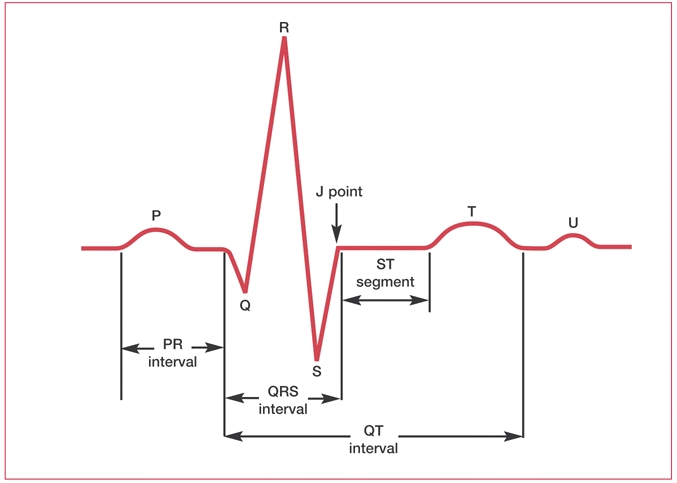
\includegraphics[width = 0.35\textwidth]{ecg_components.jpg}
\caption{\label{fig:ecg_components} Components of an ECG waveform}
\end{figure}

Typically, when looking at an ECG, clinicians will take the following characteristics into account:

\begin{enumerate}
    \item[\textbf{Rate}] The intervals between QRS complexes are considered as an indication of heart-rate.
    \item[\textbf{Rythm}] The morphology of the different components, and the intervals between them are considered to indicate any deviation from the expected/healthy sequence of operations. For example, and absence of P waves and irregular and narrow QRS complexes are an indicator for atrial fibrillation.
    \item[\textbf{Axis}] Used with multi-lead ECGs, a determination of the direction in the heart of electrcial activity, by comparing the differences in amplitude between the R and S waves on different leads.
\end{enumerate}

Deviation from the defined expected values of the above values can be indicative of specific cardiac abnormalities\cite{cardioBook}.

Taking all of this into consideration, it is clear that any single lead ECG diagnosis tool will need to at a minimum be considering the first of the above two features. The first step to accomplishing this is to identify the locations of the various waveform components.

For any model, or component of any model, that is solely making diagnoses based on the PR, RR, QT, ST intervals, we clearly must have Amplitude, and Shift invariance.

\subsection{Automated ECG Diagnosis}
Automated ECG Analysis has been extremely widely researched over the last number of decades, for a range of clinical applications. Here, we will consider a single lead ECG, generating a univariate signal/time series. The main clinical application of single led ECGs is in small long term cardiac monitoring devices, that generate very long signals, and cannot feasibly be diagnosed by hand.

Further, there are an enormous amount of cardiac defects that can be identified from ECG signals. It is outside the scope of this research to attempt to classify them all, so where we demonstrate empirical applications for clinical diagnosis, we will restrict ourselves to the example of Atrial Fibrillation, on of the most common cardiac defects.

\subsection{Characterising ECG Signals as Time Series Processes}
Here, we briefly consider what time series properties are exhibited by ECG signals, and what assumptions we can safely make about such signals.

\paragraph{Stationarity \& Homoskedasticity}
ECG signals cannot be assumed to be stationary in realistic conditions. Baseline wander is observed due to external electrical interference, as well as other biological factors such as respiratory and muscular activity. In the case of baseline adjusted signals, the mean can be assumed to be stationary, with minor variations. In neither case can the variance be assumed to be constant - the rate and rhythm of the cardiac activity will vary over the course of the ECG, and this may or may not have diagnostic significance.

\paragraph{Periodicity}
The ECG waveforms themselves are not seasonal, but variably periodic, where the inferred time series of the changes in the periodicity is of clinical significance.


\paragraph{Shift Invariance}
As a consequence of these properties, shift invariance does not perfectly apply to ECG data. Any shift invariant methods that are applied must be sufficiently robust to variations in the periodicity/heart-rate, and be applied in a windowed manner over a sufficient duration of the time series to be able to capture localised variations in the waveform periodicity.

\paragraph{Amplitude Invariance}
Due to the natural differences between patients, placement of leads, accuracy of the ECG monitoring device, degree of noise present, there is some minor variation in the voltage measured of adjacent waveforms. In an excessive degree, this may be indicative of a clinical or experimental anomoly. In the general case, however, any analysis should be robust to these amplitude variations.


\subsection{QRS Complex Detection \& R Peak Extraction}

Since the QRS wavelt is the dominant repeating component of an ECG signal, it makes sense to identify their location as the first step of a traditional automated diagnosis pipeline. \cite{ecgReview} provides a good review of methods used to perform computational QRS complex detection.

\section{A Review of Existing Approaches to QRS \& R-peak Extraction}

\subsection{Mathematically Modeling \& Characterising an ECG Signal}
Before performing any automated diagnosis of an ECG signal, we must first create some mathematical representation in which to express it. Over the many years of ECG research, the multitude of approaches have lead to some distinct methods of representing ECG signals.

\subsubsection{Combination of multiple statistical processes}
There have been some attempts to model ECG signals as well defined compositions of precisely defined processes. \cite{Napolitano2022Jan} attempts to form a very precise expression for a healthy ECG signal as an explicitly defined statistical processes. This appears to have been at least in part inspired by \cite{coupledECG} which modelled ECG signals as coupled systems of ordinary differential equations. Other similar approaches are referenced in the introduction of \cite{Napolitano2022Jan}.

\subsubsection{Combination of multiple reference wavelets}
\cite{shapeMatch2007} build a library of known wavelets within different ECG channels that correspond to certain diagnoses. It then uses DTW to determine the most relevant known wavelets to an undiagnosed signal. 

\subsubsection{Drawbacks of an explicit mathematical model or statistical process}
While being able to describe ECG signals as composition of known statistical processes would be extremely desirable, this approach has not been widely adopted (to the best of our knowledge) and is generally overlooked in recent research. 

The first reason is the large level of noise, from a variety of different sources.

 \cite{Napolitano2022Jan} states they the are working under the assumption of additive noise that is independent of the ECG signal. However, \cite{ecgNoiseReview} describes some of the most common sources of noise in ECG signals - namely baseline wander, power-line interference, and muscle artefacts. As a simple violation of the independence assumption, we might expect higher levels of muscle artefacts and baseline wander due to increased levels of respiration and movement for patients with an elevated heart rate. This would result in a noise that is correlated to the RR interval of an ECG. 

 Secondly, there is a huge amount of natural variability between healthy ECG signals for different individuals. In \cite{ecgPractice} for example, we see that S waves can sometimes be greater in amplitude than R waves in lead 1 of 12 lead ECGs (com only used for single lead ECGs). We also see that, as another arbitrary example, abnormal P waves are not indicative necessarily of cardiac defects if observed as part of  a `ectopic atrial rhythm`.

 Further, the placement of the leads will determine the axis of observation, and deviations in placements between patients will result in small relative differences between the strength of different components of the ECG signals between measurements.

Ultimately this leads to a highly coupled system of enormous complexity. There are an enormous number of potential transformations of the basic components of an ECG, whose interpretations are all strongly interlinked. Manual codification of these in a manner that is robust to uncontrollable external sources of noise is a very difficult challenge.

\subsection{Feature Extraction \& Classification Methods}
A variety methods have been proposed to identify the locations of QRS complexes, by the classification of different sets of features, broadly categorised in \cite{Gupta2021Oct} as

\subsubsection{Feature Extraction}
\paragraph{\textbf{Time domain features}}
Morphological features of the ECG considered as a temporal signal or time series. For example, this could involve the usage of matched filters, where distance measures such as DTW to known reference templates as used as features, as well as measurements of intervals between strong matches of such templates.

\paragraph{\textbf{Frequency domain features}}
These methods focus on the concentration of power in different frequencies in the Fourier Transform (or Power Spectrum) of the signal.

\paragraph{\textbf{Time-Frequency domain features}}
As a compromise between the above, these methods attempt to extract features that are compromises between the above types of information. Methods such as STFT, Hilbert-Huang transform and Wavelet analysis are used to accomplish this. Across the literature, wavelet transforms appear to be by far the most commonly applied to ECG signals of these different methods.

\cite{KAPLANBERKAYA2018216} attempts to describe more clinically specific features that can be extracted from raw signals

\paragraph*{a) \textbf{P-QRS-T complex features}}
Strongly related to Time domain features above, this category has the added restriction of features that are based on some morphological relationship between an unknown signal (or portion thereof) to a known signal representative of some \textit{known characteristic} of a reference ECG signal.

Typically, this therefore involves the use of some processing methods to identify likely Q,R,S and T peaks in an undiagnosed ECG, to generate these higher level features.
\paragraph*{b) \textbf{Statistical features}}
This refers to basic summary statistics that can be calculated on any time series - mean, standard deviation, minima and maxima, etc.

\paragraph*{c) \textbf{Morphological features}}
Distinct from P-QRS-T complex features, some methods will extract  morphological time domain feature with no underlying reference to some ground-truth clinical component of a general ECG signal. For example, \cite{polyApprox} use polynomial approximations of ECG signals as features for a diagnositc model.

\paragraph*{d) \textbf{Wavelet features}}
Due to the ubiquity of wavelet transforms in ECG diagnosis, the review overlooks features purely in the frequency domain (such as the Fourier Transform), and does not consider other time-frequency representations, such as the STFT or Hilbert-Huang Transform, and only considers the wavelet decomposition.

\subsubsection{Classification of QRS complexes \& R peaks from extracted features}
\cite{KAPLANBERKAYA2018216} also discuss the most commonly applied classification models to their aforementioned feature classes, for general ECG analysis.

\begin{enumerate}
    \item Neural Networks
    \item Linear Discriminant Analysis
    \item k Nearest Neighbours
    \item Support Vector Machines
    \item Decision Trees
    \item Bayesian Classifiers
\end{enumerate}

\cite{ecgReview} provides a review of these methods applied to the specific problem of QRS complex detection. Many of the methods applied consist of two distinct stages: preprocessing and  classification/detection.

\paragraph*{a) \textbf{Pre-processing methods}}
\begin{enumerate}
    \item Band-pass filtering
    \item Wavelet Transform
    \item Empirical mode decomposition
    \item Derivative Filtering
    \item Moving Average Filtering
\end{enumerate}

\paragraph*{b) \textbf{Detection methods}}
\begin{enumerate}
    \item Thresholding on the pre-processed signal. It is noteworthy that some of the more successful methods implemented \textit{adaptive} thresholds \cite{adaptThresh}, where a pre-defined upper and lower threshold are iteratively reduced and raised respectively until correspondence is achieved
    \item Neural Networks applied to the raw signal
    \item Hidden Markov Models on the pre-processed signal
    \item Syntactic pattern recognition on the raw data. This is similar to HMM models, and the previously mentioned methods to explicitly model the different components of ECG signals
    \item Moving Average Filtering
    \item Zero Crossing detection on the pre-processed data. This is particularly relevant when applied to derivative filters, and when used with wavelet transformations, due to the large gradient changed on the RS and QR intervals.
    \item Genetic Algorithms
    \item Singularity point detection - similar in practice to Zero Crossings on wavelet transforms, singular points are those which have derivatives of opposite signs to the left and right \cite{singularECG}  
\end{enumerate}

This review noted that the Neural Network models were particularly noise sensitive.

More recent studies, such as \cite{dogan_dogan_2023} (published only a week before the time of writing), we still see that the most advanced neural network models which, with much higher levels of computational complexity, achieve at-best marginal improvements over well established filter-and-threshold based methods.

\section{Characterising \& Contrasting Approaches to QRS \& R-peak Extraction}
It is notable how much neural network models have struggled to match the performance of extremely low-complexity models, while retaining a much more noticeable degree of sensitivity to noise.

Here, we will consider the underlying structure of a simple wavelet decomposition \& threshold based model, compared to a simple 1-Dimensional CNN model. We will determine what the fundamental capabilities of these are, and what the consequences are for their relative  performances.  

\subsection{Contrasting wavelet and CNN methods}
It is particularly interesting to note the relative success of wavelet \& threshold based methods over CNN methods, considering their apparent structural similarities.

Most wavelet decompositions consist of levels of consisting of high-pass filters and decimation (usually by a factor of 2, for a so-called d\textit{Dyadic} wavelet decomposition). This is followed by thresholding at each level of \textit{coefficients}, and recomposition with low-pass filters and up-sampling.

These filters are computed analogously to the kernel convolutions in CNN models, and the architecture of a wavelet decomposition is very similar to that of a CNN auto-encoder, with modified residual connections. Indeed, there have been some wavelet based CNNs that are specifically architected to resemble wavelet transforms, such as \cite{despawn}.

Even though these architectures are so similar, CNN models require vastly more complexity to reach similar levels of performance, and even that, at lower levels of robustness. Therefore, there is at least one component of the simple wavelet \& threshold model that CNN models struggle to capture - either the capability of the wavelet transform to accomplish effective feature extraction, the capability to learn an effective decision boundary on the extracted features, or the capability to perform both jointly.

\section{Generalising R Peak Extraction}
In order to assess the general capabilities of these differing approaches, we will consider the general problem of R peak extraction, as pertains to an abstract time series. The characterisation of an ECG as a general time series is described in section II-G.

We can consider ECG signals as having approximately constant mean, variable periodicity, variable amplitude across periods, and exhibiting highly complex non-stationary noise that has a trend, cycle, and may be partially correlated to some clinical properties of the signal. The most important aspect of this is the noise, which is challenging to deal with.

R peak extraction can be considered on such a general series to be the process of isolating the positions of the highest amplitude component of the variably periodic wavelets of the signal. Take note that this may not be the actually observed highest amplitude component of an observed signal, and further, the highest amplitude component of an observed signal may not correspond to a true peak. Our definition of a peak, is that of the true maximum, generated by some characteristic of the underlying process of the time series, that can be observed in a perfectly noiseless signal. Obviously, even the best prediction model will generate false detections in the presence of sufficiently strong noise.

Such a model should output a sequence of 0/1 values corresponding purely to presence/non-presence of this component at a given time point in the signal - this output should be of uniform amplitude. In the case of R peak extraction, wavelet models often explicitly incorporate prior knowledge about expected intervals on these predictions, and it is assumed that neural network models will implicitly learn these distributions. However, we will drop this component from our general model, to allow for broader conclusions. Henceforth, we will refer to this generalised problem as peak amplitude detection, to create a distinction from the specific instance of R peak extraction. 

\subsection{Characterising Peak Amplitude Detection}

The ideal peak amplitude detector, which perfectly identifies peak amplitudes for all possible input signals observes the following invariances, at a minimum:

\paragraph{Conditional Amplitude Invariance}
The restriction of the model to purely positional information (1/0) outputs is in fact a form of conditional amplitude invariance. The detector must effectively create two sets of decision spaces, where an observation, or set of observations falls into one set or the other, corresponding to peak amplitudes or non-peak amplitudes. The model is obviously, by design, invariant to local variations between observations in the same set. An example of this can be seen with models based on thresholds - the threshold creates a decision boundary that delineates the sets of peak and non-peak amplitude observations.

\paragraph{Shift Invariance}
The operation of peak amplitude detection must clearly be shift invariant - a peak should be deetected regardless of the overall phase of the input data.

If a method does not exhibit these characteristics, it will not be \textit{robust} to irrelevant variation input data, no matter its level of complexity or degree of optimisation. This problem should also incorporate Local Scale, Uniform Scale, Complexity invaraince, but these will not be as important in the following discussions.

\section{Contrasting Deep Learning and Wavelet Methods for Peak Amplitude Detection}


\subsection{Assessing both Methods for Shift Invariance}

By the mechanism of the convoluational/cross-correlational operations that are equivalent across wavelet and CNN models, it is easy to see that these operations are shift invariant. However, downsampling in both approaches will result in violation of shift invaraince.

Downsampling in traditional signals processing is typically performed by taking the average over consecutive disjoint sets of values, to correspond to a single value in the downsampled signal. E.g., pairs of adjacent values can be averaged to correspond to a downsampled signal of half the length of the input.

In the case of wavelet transforms, the low pass filter has an anti-aliasing affect, which mitigates the effect of the shift variance of the downsamplign operation. \cite{bradley2003shift} However, with increased thresholding, this breaks down, allowing shift variance to creep in. However, a modified wavelet transform, the \textit{algorithme à trous}, can achieve shift invariance with equivalent predictions. It does this by expanding, or dilating, the filters by 0 padding between elements, at each level instead of downsampling the signal.

Similarly, for CNN models, the pooling operation is not shift invariant. However, there is a modification of CNN models to achieve better shift invariance known as a dilated CNN, which are analogous to the algorithme à trous in terms of dilating the kernels rather than downsampling the input data.

Therefore, for a general truly shift invaraint operation, particularly such as in this instance, where we wish to precisely locate a feature to within a single sample, these dilated filter operations are much preferable.

\subsection{Assessing Wavelet Methods for Conditional Amplitude Invariance}

The conditional amplitude invaraince is achieved trivially with hard thresholds in the wavelet decomposition models - where the construction of the 1/0 outputs is explicitly coded into such models. However, there are two slightly different types of conditional amplitude invariance achieved, depending on whether the thresholds are pre-defined as specific amplitude values, or relative - where the thresholds are computed as a certain percentile of the observations. Adaptive thresholds are a slight modification of relative thresholds, where independent thresholds are computed over subsections of the data.

\paragraph{Global Thresholds}
For a fixed, pre-defined threshold, the outputs are invariant to variations in the inputs that do not cross the threshold. Said different, it is invariant to localised variations on either side of the decision boundary.
\paragraph{Relative \& Adaptive Relative Thresholds}
For a relative threshold, the outputs are amplitude invariant - multiplying the entire signal by a constant factor will not affect results. It also demonstrates the same conditional invariance as global thresholds, where the outputs are invariant to variations within the lower and upper precentiles that do not alter the computed threshold position.

\subsection{Assessing CNN Models for Conditional Amplitude Invariance}

The main mechanism by which a CNN model can form a decision boundary for 1/0 classification, from some arbitrary weighed output, is by use of non-linear activation functions. Here, we will first consider which properties of an ideal peak amplitude detection model are exhibited by an individual activation function. Then, we will generalise this to compositions of activation functions to better reflect a full deep model.

\paragraph{Activation Function Properties}
Traditionally, many activation functions used in neural network models, such as tanh and sigmoid activation functions closely resemble soft-threshold functions. The Heaveside step function, or true threshold, has long been proposed for different deep models, but rarely applied to due the impossibility of training by gradient descent.

It can be easily shown that any activation function that has bounded outputs will experience vanishing gradients in the upper and lower limits.

Let  $f\left(x\right)$ be an arbitrary monotonic function. We will not consider activation functions that are not monotonic in the limit, as these have no practical benefits. Let us assume $f$ is monotonically increasing, with domain $\left[a,b\right]$.

$ \implies \lim\limits_{x\to -\infty} f\left(x\right) = a, \lim\limits_{x\to \infty} f\left(x\right) = b $

Using Newton's Quotient as an estimate of the derivative of $f$:

$f^\prime\left(x\right) = \lim\limits_{h\to 0}\frac{f\left(x+h\right)-f\left(x\right)}{h}$

However, under the limit $x \to \infty, \left|f\left(x\right)-f\left(x+\delta\right)\right|=0$, by construction of $f$

$\implies f^\prime\left(x\right) \approx \lim\limits_{h\to 0}\frac{f\left(x\right)-f\left(x\right)}{h} = 0$ as  $x\to \infty $

Clearly, any fully bounded function has a 0 derivative in the upper and lower limits - causing a vanishing gradient that kills optimisation.

Further, as the activation approaches a perfect decision boundary, with outputs approach perfect segmentation into exact $a$ and $b$ values, the gradients approach 0. This is a straightforward consequence of the well known vanishing gradient problem.

A common approach to address vanishing gradients in activation functions such as ReLU is to remove the bounds on the function, and enforce a lower limit on the gradient of the function. It is easy to intuit, and demonstrate, that the higher the lower bound on the gradient, the more the bounds on the original function are violated

Here, we will assume that $f\left(x\right)$ crosses the x-axis at (0,0) without loss of generality

Assume that, in order to address the vanishing gradients of $f$ previously demonstrated, we impose a lower bound on the gradient of $f$ - $\text{min } f^\prime\left(x\right)=\delta_\text{min} \; \forall x\; \in\left[0,\infty\right]$

Considering  $\;f$ on $x\;\in\;\left[0,\infty\right]$, monotonically increasing, a lower bound on $f\left(x\right)$ is $f\left(x\right)=\int_0^x\delta_{\text{min}}\text{dx}=x\delta_{\text{min}}$

In the best case, the bounds of $f$ therefore linearly increase with the inputs.

We can thus further elaborate on our tradeoff - as the gradient-based trainability of a particular function increases, its ability to define a true decision boundary at best linearly decreases.

\paragraph{Activation Function Trainability/Bounding Tradeoff}
As a consequence, there is a fundamental inability for an activation function's ability to form a conditionally amplitude independent binary classification threshold.

If such a threshold exists, with outputs that are equal to some upper bound and lower bound value, this activation function must have a 0 gradient, making it untrainable by gradient-based optimisation.

Here, we define gradient-based optimisation as any optimisation method which uses any objective function that consists of some multiple of the activation function's gradient $f^\prime\left(x\right)$.

Trainability of these activation functions is only possible when:

\begin{enumerate}
    \item The outputs of the activation functions are distributed between $a$ and $b$, at a significant distance from the upper and lower limits. 
    \item The activation function is unbounded
\end{enumerate}

In both cases, we are in violation of the conditional amplitude invaraince, as local variations within each decision set (above and below the decision boundary), generate different outputs. 

\paragraph{generalisation to a multi-layer network}

Above, we have only considered the case of a single activation function. The situation is slightly different when considering a multi-layer network, but we will see that similar properties hold.

Firstly, let us briefly consider the case where the bounded decision-boundary classification function $f(x)$ is composed of multiple non-linear functions which may not necessarily individually have vanishing gradients on different intervals, $f(x)=h\circ g(x)$.

Letting $y = h\circ g(x) = h(g(x))$, assume $\displaystyle \frac{\delta y}{\delta g}$  not necessarily have a vanishing gradient. $\displaystyle \frac{\delta y}{\delta x} =  \frac{\delta y}{\delta g(h(x))} \times \frac{\delta g(h(x))}{\delta h(x)} \times  \frac{\delta h(x)}{\delta x} = f^\prime(x)$ by the above argument, will still experience vanishing gradient. Thus, while the lower layers of this network might train under such an ideal instance, any jointly optimised pre-processing components acting as inputs will become untrainable, as this decsion boundary becomes more optimal.  

As an overall consequence, the more accurately any neural network model becomes at forming a true decision boundary that is robustly invariant to noise above and below the boundary, the less trainable this network will become.

\paragraph{Batch Normalisation}
A extremely prevalent method to address vanishing gradients in deep models is the use of normalisation. This is typically applied over batches, although weight and layer normalisation have also been proposed and applied in some instances.

\cite{invariantsWithDNN} (as a rare piece of research into deep models that respect time series properties) notes that normalisation is not always appropriate for time series modelling for deep learning. This is due to the lack of a known supremum and infimum for a time series, and lack of stationarity. 

Here we will consider the case of an approximately stationary time series, where batches consist of adjacent or overlapping windows of observations for maximal consistency within batches. We will also assume that outlying extrema are either not present, or extremely rare in the series.

In this instance, we will consider what improvement, if any, will normalisation lend to the aforementioned issues with trainable and robust decision boundaries.

Batch normalisation, as defined in \cite{invariantsWithDNN}, is
\begin{equation*}
    \mu_B = \frac{1}{m}\sum_{i \in \left[1,m\right]}x_i, \sigma_B^2 = \frac{1}{m}\sum_{i \in \left[1,m\right]}\left(x_i-\mu_B\right)^2
\end{equation*}
\begin{equation*}
    \hat{x_i} = \frac{x_i-\mu_B}{\sqrt{\sigma_b^2+\epsilon}}, y_i = \gamma\hat{x_i}+\beta
\end{equation*}

Where $\gamma$ and $\beta$ are scaling and centering parameters.

Normalisation results in output data that has mean of 0 and variance of 1, but makes no guarantees about the bounds of the data. As a result of the reduced variance, there is decreased likelihood of experiencing vanishing gradients on continuous and monotonic activation functions, however, this clearly leads to poorer distinction of outputs into exact values. As a consequence, this does not have any bearing on the trainability/thresholding tradeoff discussed above.

Overall, normalisation results in amplitude invariance for any decision boundary that is applied to such normalised data. While this suggests that batch normalisation may be therefore allowing us to construct decision boundaries that are similar to relative thresholds, this is not exactly the case. Since this is based on the varaince of the data, rather than scaling based on \textit{percentiles} of the data, we can find that regular decision boundaries approximated on this data are not robust to variations in amplitude above and below certain percentiles. In order for the normalisation to result in better conditional amplitude invaraince of any learned decision boundary - in other words, to convert a global threshold to more closely resemble a relative threshold, the normalisation should be applied using the variance of only specific percentiles of the input data.


\subsection{Consequences for peak amplitude detection with Nueral Netowrk models}

\begin{enumerate}
    \item It is impossible for a model to be fully trainable for both pre-processing and threshold based classification, while also achieving robust amplitude invariant classification outputs that are invariant to local variations above and below the classification boundary
    \item For the approximated decision boundary to approximate a relative threshold, performance may potentially be improved by performing normalisation independently on different percentiles of the data 
\end{enumerate}

It is very important to note that these limitations apply to internal representations of complex neural network models, not just the outputs of simpler models. Specifically, point 1) above shows that any neural network that attempts to extract purely positional representations of the peak amplitude component of a periodic signal, will not be trainable unless this representation has a certain degree of sensitivity to amplitude varaitons and nosie.

\section{Consequences for R peak extraction}
In the specific instance of R peak extraction, it is a consequence that any neural network model that attempts to identify purely R peak locations, with outputs that are totally independent of amplitude information will have to balance robustness with trainability.

For a neural network model to achieve trainability on this data, it must sacrifice the ability to construct a robust, conditionally amplitude invariant decision boundary. 

For models that are trainable, and manage to achieve accurate performance on this data - they are doing so in a manner that is therefore not robust to localised variations in amplitude. As a consequence, it is extremely likely that under different experimental setups, such models by their very nature will produce more inconsistent results. It is possible that an extremely high degree of complexity is required in these models to account for a multitude of different noise and amplitude characteristics in order to attempt to eliminate them by filtering without direct application of a decision boundary. 

As an exemplar methodology, for putting theoretical derivations such as those above into practic, we will consider a lightweight deep model that has performance equivalent to that of a simple wavelet \& threshold based method.

Due to the pre-exisitng similarities between these methods, we are going to consider one potential CNN architecture that reflects the structure of a wavelet decomposition as much as possible, and attempts to observe the principles discussed above as much as possible

\begin{enumerate}
    \item The residual connections should be organised in order to resemble a wavelet decomposition as closely as possible. It may also be beneficial to constrain the weights to have properties that are derived from the filters used in wavelet decompositions
    \item Downsampling should be achieved with dilated kernels, rather than pooling
    \item Activation functions must be chosen to balance trainability with thresholding capability
    \item If batch normalisation is applied, it should be performed with batches consisting of adjacent or overlapping samples. It may also be beneficial to perform the normalisaion based on the variance of only a certain percentile of the data, to allow better correspondence to an adaptive threshold
\end{enumerate}
\section{Empirical Experimental Setup}
\subsection{Dataset}
The MIT-BIH dataset\cite{dataset} was chosen, due its prevelance in the literature, as well is its convenient clinician-verified annotations of the R peaks (and other features). This data is taken from 2 lead ECGs, only the signal from the first lead was retained for the trainaing/validation phase.

\subsection{Hardware \& Software}
All models were trained between two machines with the following specifications

\begin{enumerate}
    \item  Intel Core i7-1165G7, 16GB RAM, RTX 3060 eGPU
    \item  Intel Core i7-6800K, 16GB RAM, GTX 1080
\end{enumerate}

Deep models were implemented using TensorFlow 2.10.1 on Python 3.10. Implementations are available at \url{https://github.com/andrew-nash/fyp}

\subsection{Experimental Testbed}

\section{Empirical Experiments}
\subsection{Threshold/trainable compromising activation function}
In order to better balance the tradeoff between trainability (by lack of vanishing graadients), and thresholding capability, we propose the \textit{Triple Linear Activation} - that attempts to achieve a better (and more finely adjustable) balance between these factors than common activation functions.

\begin{figure}
    \centering
    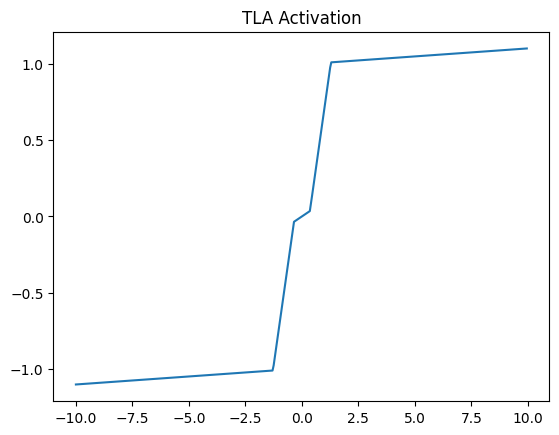
\includegraphics[width=0.35\textwidth]{tlaAct.png}
    \caption{the proposed activation function}
\end{figure}

The proposed function is a simple piecewise linear approximation of a sigmoid or tanh pattern activation function, with a guaranteed minimum gradient at all points. This minimum gradient is left as a paramater that can be adjusted by the user. At lower values, this function closely approximates a hard threshold, but will experience vanishing gradients. At higher values,  the minimum gradient increases, but the thresholding capability is lost.

\subsection{Validating the principled approach}
In order to provide a demonstration of the practical utility of our general theoretical observations for time series modelling with deep models, we demonstrate a model for R peak classification that takes these observations into account. We compare this against the results of a more traditional unprincipled model tat is structurally similar to the current state of the art deep models for ECG analysis.

All training was done on batched data, with batches consisting of two adjacent samples of an ECG signal. The exact details of each architecture are shown in Appendix A.


\paragraph{\textbf{Conventional Deep Learning Model}}
As a baseline, we implemented a 1 dimensional Residual CNN model, based on \cite{stanfordML}. This reflects the current state of the art for ECG analysis.




\paragraph{\textbf{Wavelet Inspired Deep Learning Model}}
As a demonstration of principled model design, we propose a deep learning architecture that should, while similar in nature to the prior model, generate predictions that are more robust to local variations in the noise and R peak amplitudes. This model will consist of a residual CNN model, with a few key differences to that mentioned previously.

By our above discussion, in a traditionally architected and optimised deep model, this is inherently impossible to achieve while still being trainable. 

The proposed architecture, and the basis for the choice of each component is as follows:

\begin{enumerate}
    \item The model will incorporate an auto-encoder style model, with a block of convolutional operations followed by a block of de-convolutional on the data
    \item To better preserve shift invariance, this model uses dilated filters rather than pooling to achieve the downsampling effect in the autoencoder
    \item The ReLU activations are replaced with our proposed activation above that attempts to trade-off  trainability and thresholding capability
\end{enumerate}

\paragraph{\textbf{Wavelet Based Deep Learning Model}}

In order to further validate our approach, we will implement a much more aggressively simplified deep CNN model that almost identically resembles the structure of a wavelet transform.

This is based partially on the implementation from \cite{despawn}. This is very similar to the previous model, with the main differences being

\begin{enumerate}
    \item The elimination of BatchNorm and Dropout
    \item The limitation to a single filter per CNN layer
    \item The use of pooling rather than dilation to correspond to a true wavelet (rather than  à trous) transform
\end{enumerate}

We also fitted a derivative of this model, where, the re-composition filters were not learnable, but acted as the reverse alternate flip of the decomposition filter, as per \cite{despawn}.

The fitting of models b) and c) above requires more hyper-parameter optimisation, particularly around the choice of minimum gradients in the activation functions.

For this reason, a series of lower-complextity wavelet models were fitted on the data, and cross-validated metrics were used to identify the appropiate sets of hyper-parameters to develop a model of similar scale to the conventional ResNET.

\clearpage

\subsection{Model Summaries}

All models were fitted with homogeneous batches of 2 ECG samples of length 4096 signals (sampled at 360Hz). Models were trained with 10 fold cross validation (folds are randomised between models), for 50 epochs per fold. Input data were normalised for all models. Model losses were computed as binary corssentropy to the true 1/0 R peak positional series.

Kernel sizes were held at 16 for simplicity, and allow for fairer comparability between models. 64*(block index) kernels were fit for each convolutional operation in each block for the standard ResNET. 8 kernels were similarly fit in the Wavelet style model. The pure wavelet model fit a single kernel per convolutional layer. 

\begin{center}
    \begin{tabular}{ |p{3cm}||p{3cm}|p{3cm}|p{3cm}|  }
     \hline
     \multicolumn{4}{|c|}{Table 1: Details of fitted models} \\
     \hline
     Model Class& Residual Blocks/Decomposition Levels & Activation Gradient Parameter & No. Trainable Parameters \\
     \hline
     \multirow{4}{4em}{Standard ResNET}  & 1   & - & 198\,272 \\
                                        &   2  & -& 723\,328   \\
                                        & 3 & -& 2\,100\,672\\
                                        & 5 & - & 8\,985\,088\\ 
      \hline
      \multirow{6}{4em}{Compact Wavelet Style ResNET}  
                                        & 3 &  0.01 & 21\,041\\
                                        & 5 & 0.01 & 90\,475 \\
                                        & 3 &  0.05 & 21\,041 \\
                                        & 5 & 0.05 & 90\,475\\
                                        & 3 & 0.5 & 21\,041 \\
                                        & 5 & 0.5 & 90\,475\\
        \hline
        \multirow{9}{4em}{Traditional Wavelet}  
                                        & 2 &  0.01 & 133\\
                                        & 5 & 0.01 & 328 \\
                                        & 7 &  0.01 & 458 \\
                                        & 2 &  0.05 & 133\\
                                        & 5 & 0.05 & 328 \\
                                        & 7 &  0.05 & 458 \\
                                        & 2 &  0.1 & 133\\
                                        & 5 & 0.1 & 328 \\
                                        & 7 &  0.1 & 458 \\
                                     
        \hline

        \multirow{5}{4em}{Shared QMF}  
                                        & 2 &  0.01 & 37\\
                                        & 2 &  0.05 & 37\\
                                        & 2 &  0.075 & 37\\
                                        & 5 & 0.01 & 88 \\
                                        & 5 & 0.05 & 88 \\                          
                                     
        \hline
    
    \end{tabular}
\end{center}


\subsection{Empirical Experiment Results}

The first and most obvious comparisons to make between models are between the cross validated prediction losses.

\begin{figure}[H]
    \centering
    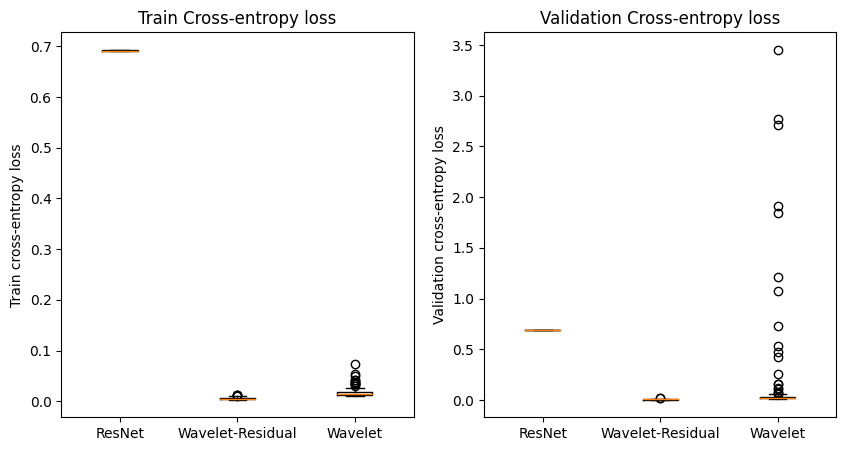
\includegraphics[width=0.5\textwidth]{full_loss.png}
    \caption{Cross validated Cross-entropy loss on the models in Table 1}
\end{figure}

\begin{figure}[H]
    \centering
    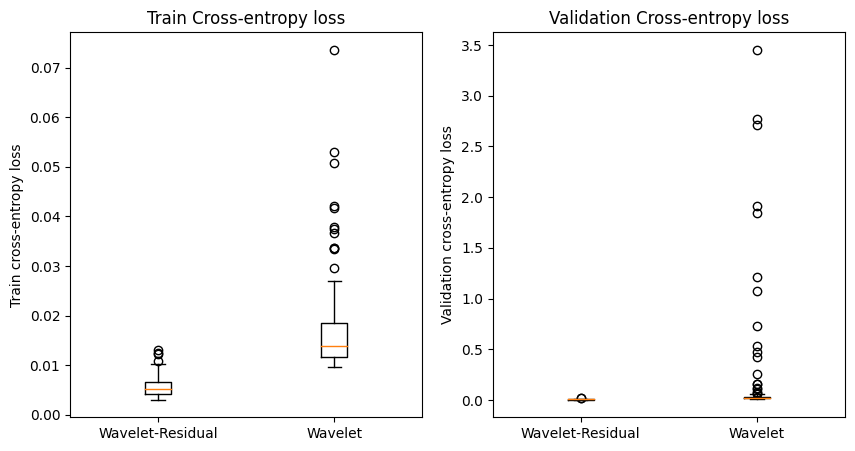
\includegraphics[width=0.5\textwidth]{full_wavelet_loss.png}
    \caption{A clearer view of the differences between teh predictions on the wavelet based models in Fig 3.}
\end{figure}

While initial indications are that the wavelet models vastly outperform the ResNET model, even though they involve vastly fewer parameters, the situation is more nuanced.

Before this can be addressed, we need to address the greater variability between the wavelet based models than the ResNET models. This is to be expected, since the hyperparamters were more varied over these models - it is therfore appropriate here to select a well performing set of hyper-parameters, and proceed to perform further comparisons with this limited set of models. This should result in fairer and more appropriate comparisons between model classes.

To do this, we will consider the cross-validated prediction losses of the models within each class, and select representative well-performing subsets of each class accordingly.


\begin{figure}[H]
    \centering
    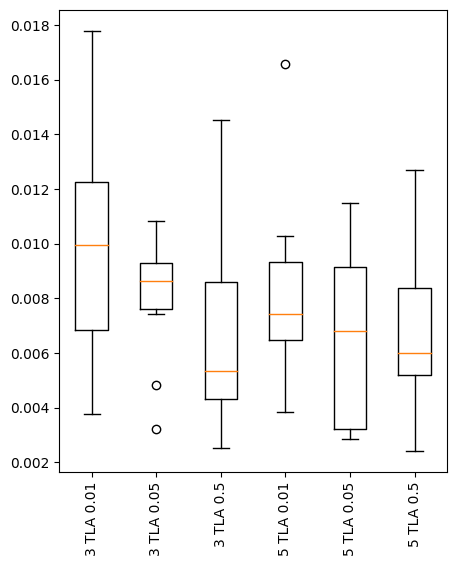
\includegraphics[width=0.2\textwidth]{waveletStlyeParams.png}
    \caption{Overall validation losses for wavlelet based ResNET implementations}
\end{figure}

\begin{figure}
    \centering
    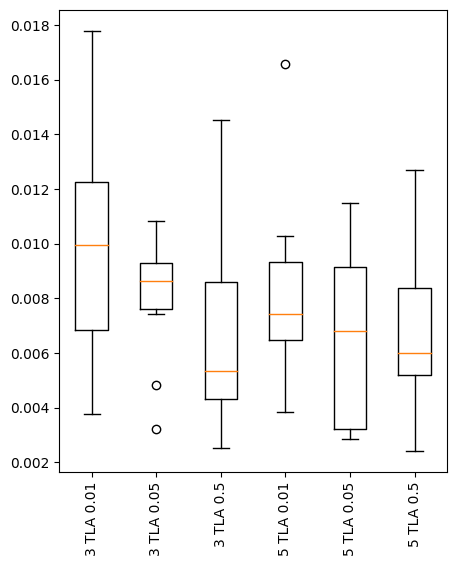
\includegraphics[width=0.2\textwidth]{waveletStlyeParams.png}
    \caption{Overall validation losses for standard ResNET implementations}
\end{figure}


\begin{figure}
    \centering
    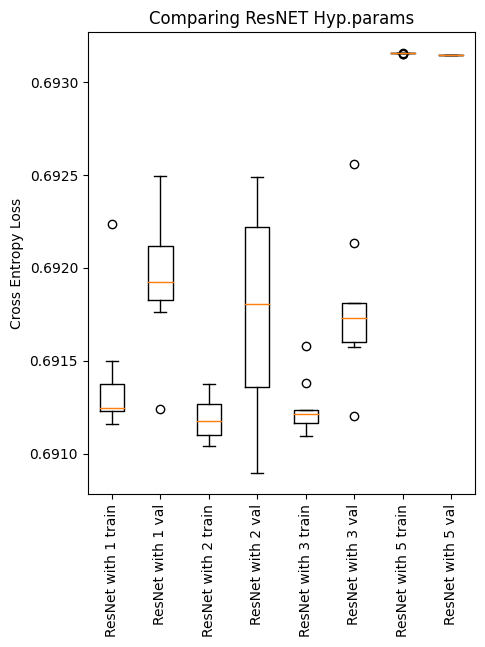
\includegraphics[width=0.35\textwidth]{resnetParams.png}
    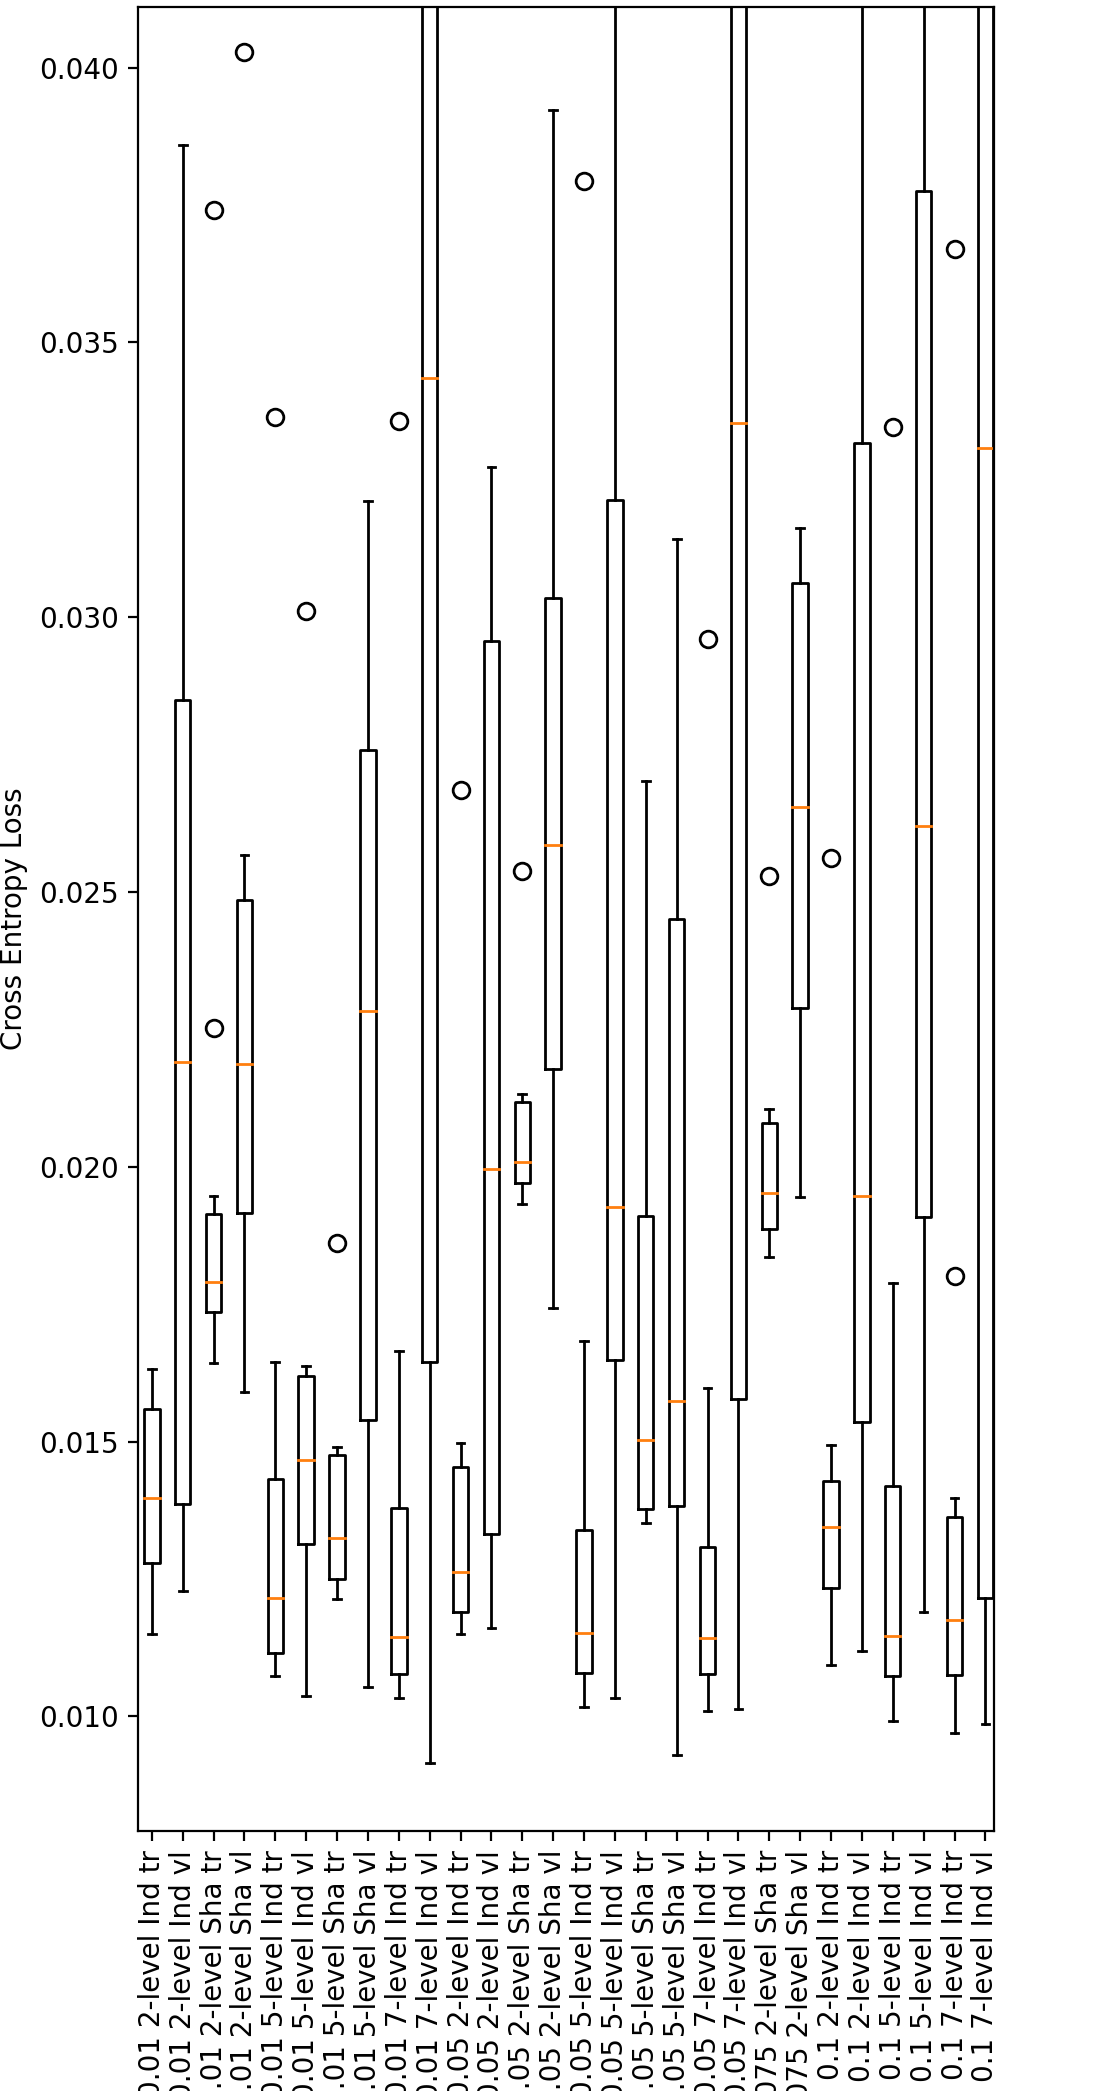
\includegraphics[width=0.35\textwidth]{waveletParamLossesDetail.png}
    \caption{Overall validation losses for simple wavlelet implementations. (Zoomed detail on right)}
\end{figure}

\clearpage


\subsubsection{Model Selection}

We do not take a rigorous and exacting model selection approach here to find the exact highest performance of some metric. The reason for this is two-fold:

\begin{enumerate}
    \item We wish to avoid overly overfitting to random variation in the validation losses
    \item The exact losses of our final model are not the important aspect of this experiment - the general performance differences between the different classes are what interests us here. The performance differences of typical, not necessarily optimally parameterised, models suffice to explore these differences between model classes
\end{enumerate}

As a general observation on the plots, models with 5 wavelet coefficients and an activation gradient parameter of 0.05 achieve consistently low losses, albeit not necessarily the absolute lowest in each model class. For consistency, however, based on this observation, further evaluation of results will be restricted to the models listed in Table 2.

\begin{center}
    \begin{tabular}{ |p{3cm}||p{3cm}|p{3cm}|p{3cm}|  }
     \hline
     \multicolumn{4}{|c|}{Table 2: Details of fitted models} \\
     \hline
     Model Class& Residual Blocks/Decomposition Levels & Activation Gradient Parameter & No. Trainable Parameters \\
     \hline
        \multirow{2}{4em}{Standard ResNET}  
                                        &   2  & -& 723\,328   \\
                                        & 3 & -& 2\,100\,672\\
      \hline
      \multirow{2}{6em}{Wavelet Style ResNET}  
                                        & 5 & 0.05 & 90\,475 \\
                                        & & & \\
        \hline  
    \multirow{2}{6em}{Wavelet Style ResNET}  
                                        & 5 (32*layer index kernels per layer) & 0.05 & 1\,406\,299 \\
                                         & & & \\
        \hline
     \multirow{3}{7em}{ResNET-Wavelet, Non-QMF}  
                                    & 5 & 0.05 & 328 \\
                                     & 5 & 0.01 & 328 \\ & & & \\
    \hline

    \multirow{3}{6em}{Traditional Wavelet - QMF Filters}  
                                    & 5 & 0.05 & 88 \\
                                     & 5 & 0.01 & 88 \\
                                     & & & \\
    \hline
    \end{tabular}
\end{center}



\subsubsection{Comparing Losses on the R peaks and non-R peaks}



\begin{figure}[H]
    \centering
    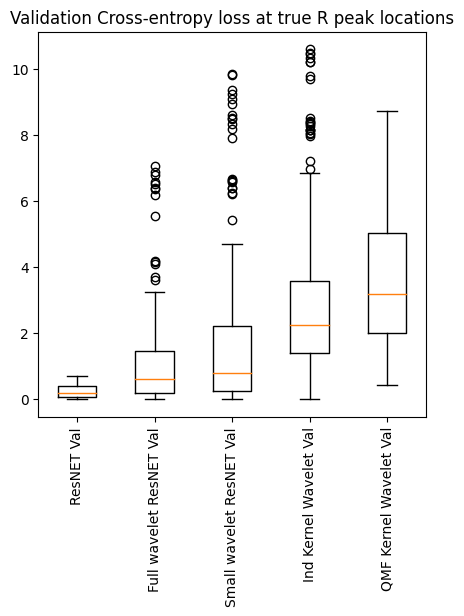
\includegraphics[width=0.3\textwidth]{valLossAtRBoxplots.png}
    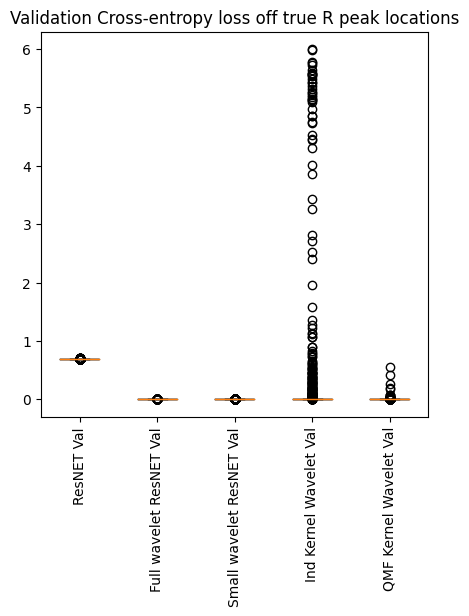
\includegraphics[width=0.3\textwidth]{valLossOffRBoxplots.png}
    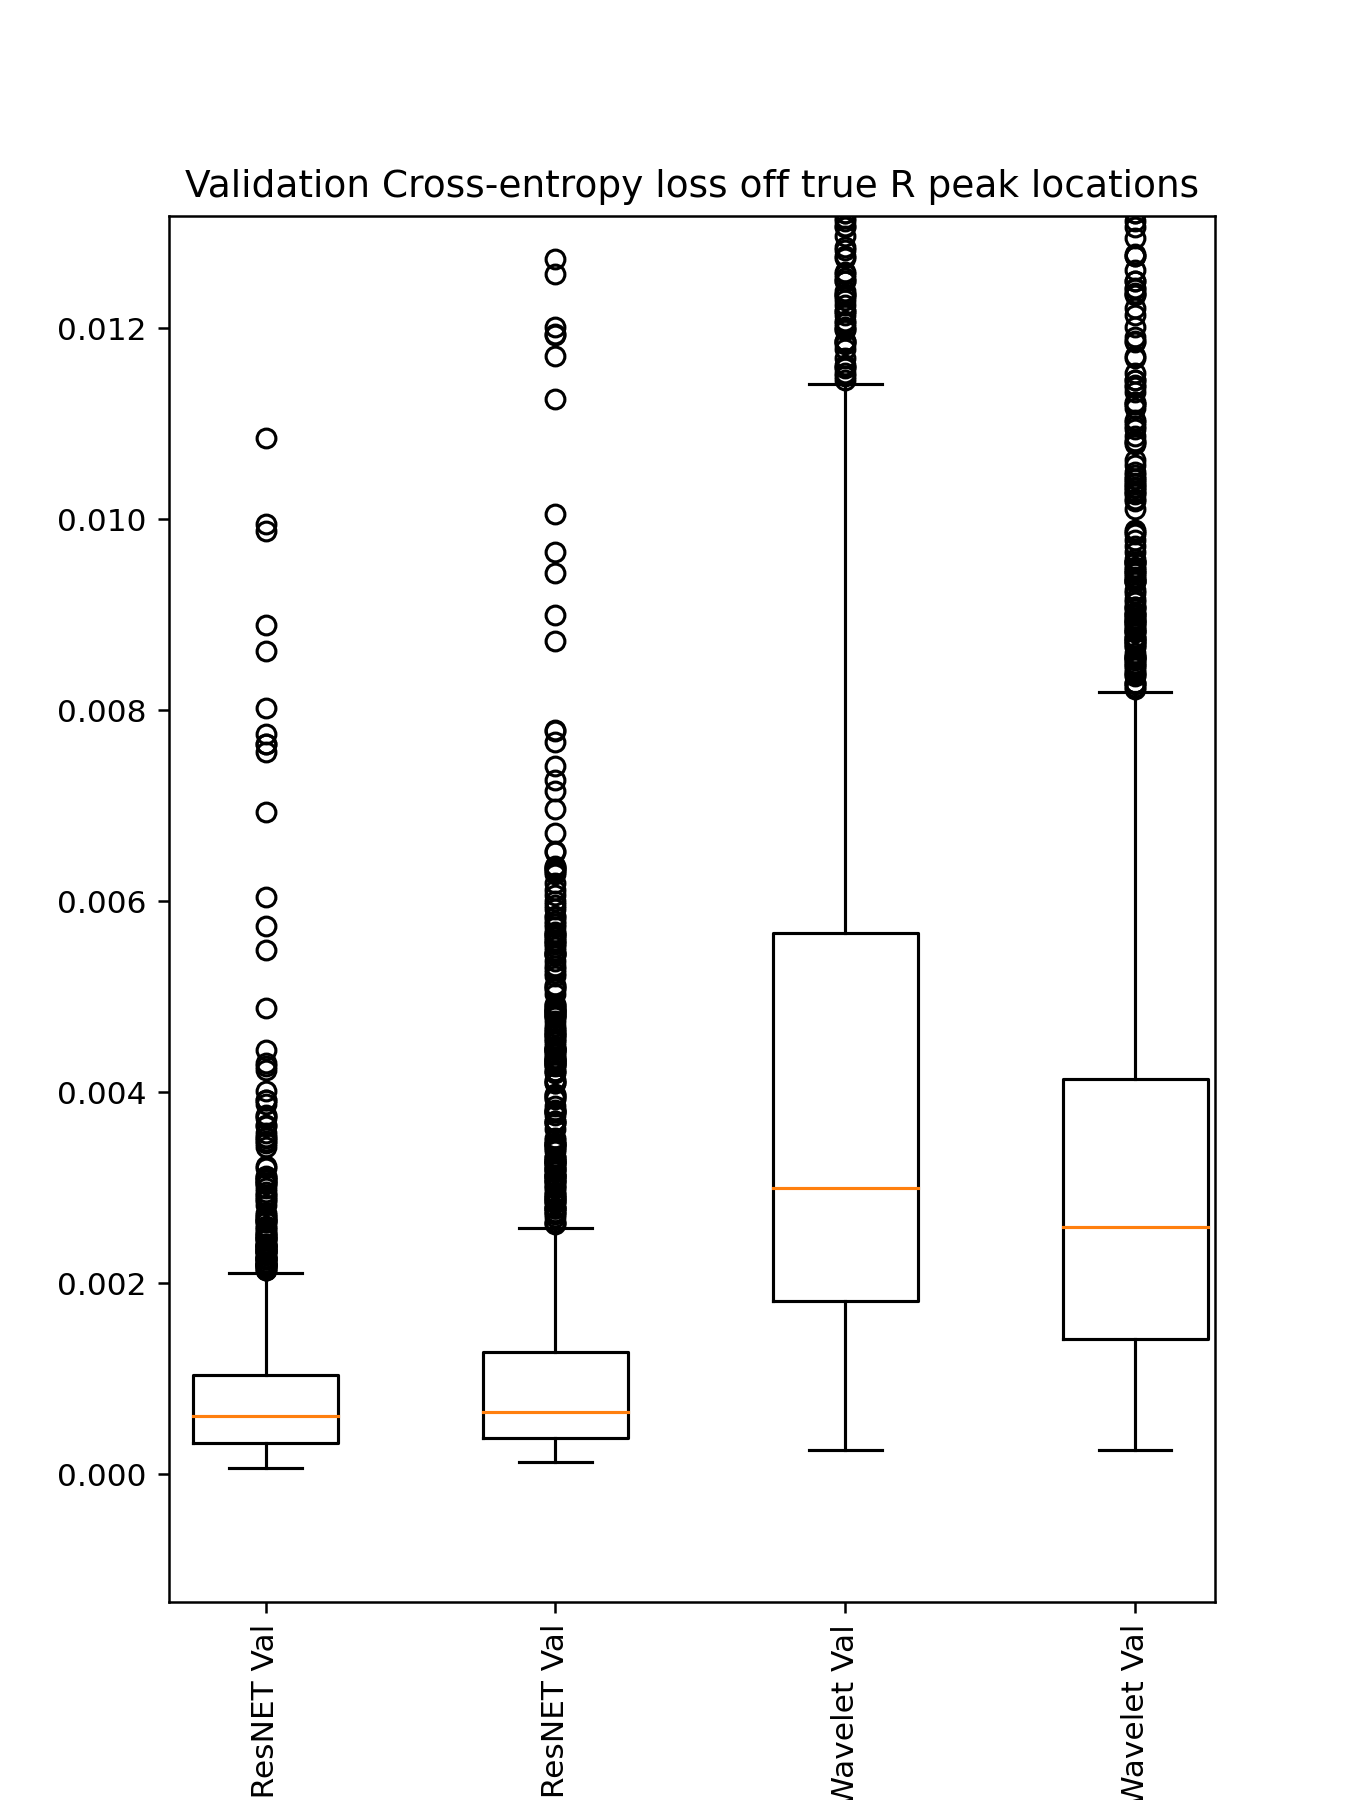
\includegraphics[width=0.3\textwidth]{valLossOffRBoxplotsZoomed.png}
    \caption{Validation loss at R peak and non-R peak points. All models correspond to those listed in. Rightmost plot is a zoomed section of the centre plot that better illustrates the differences between the last 4 boxes.}
\end{figure}



Interestingly, separating the loss into the components of loss incurred by true positives and true negatives serves to better differentiate the performances of the different models. 

The first immediate observation here is that the prediction loss declines for the less sophisticated wavelet based models. For this reason, we will initially consider only the differences in performance between the standard and wavelet style ResNET/residual models. We will revisit the other wavelet models in a further section.

\paragraph{\textbf{Comparing Performance Between Standard and Wavelet ResNET}}
In the plots of the cross validated losses for the standard and wavelet ResNET, we see that the validation losses are lower for the standard model when considered solely on the true R peaks, and lower for the wavelet model on the other portions of the input signals. Both of these differences are found to be statistically significant by a Mann-Whitnet U test (R peak validation losses are significantly lower for the wavelet ResNET, non-R peak validation losses are significantly lower for the standard ResNET) at $p=0.05$ level of significance.

Further, Man-Whitney U tests also indicated that 

\begin{enumerate}
    \item Mean R peak \textit{prediction values} (\textbf{not losses}) are significantly lower for the standard ResNET
    \item Mean non-R peak \textit{prediction values} are significantly lower for the wavelet ResNET
\end{enumerate} 

This can be easily visualised by examining the distributions of the cross-validated prediction values for the different model classes.

\begin{figure}[H]
    \centering
    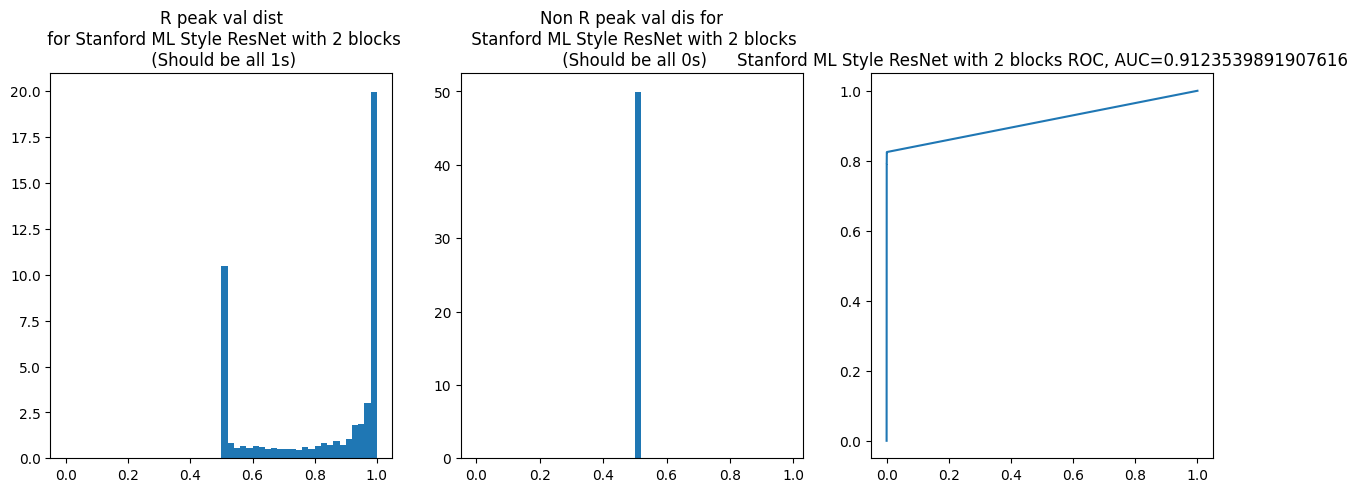
\includegraphics[width=0.75\textwidth]{resnet2Dist.png}
    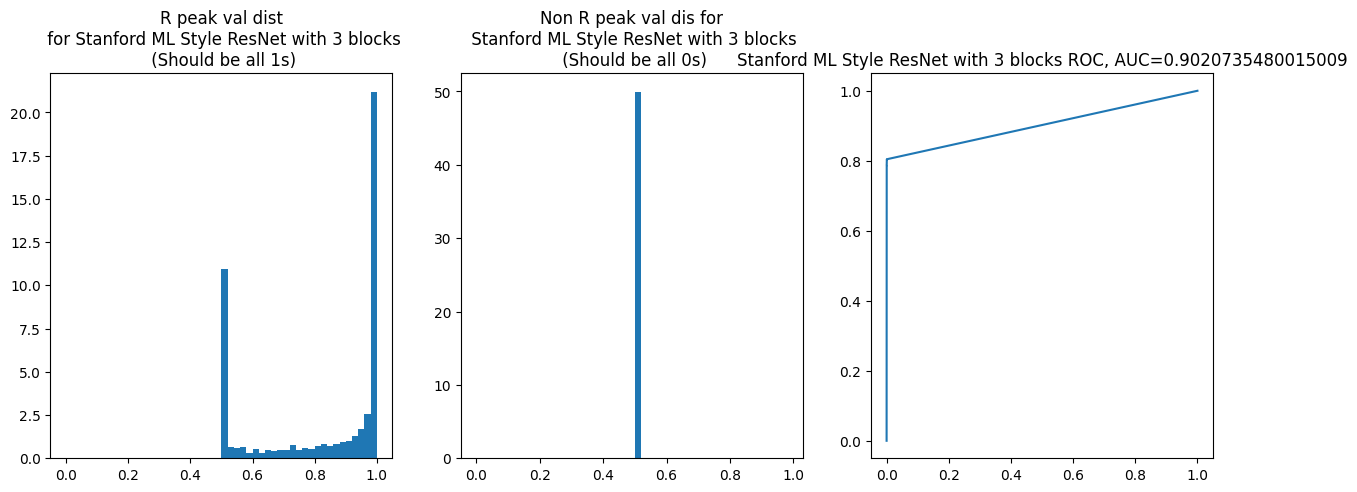
\includegraphics[width=0.75\textwidth]{resnet3Dist.png}
    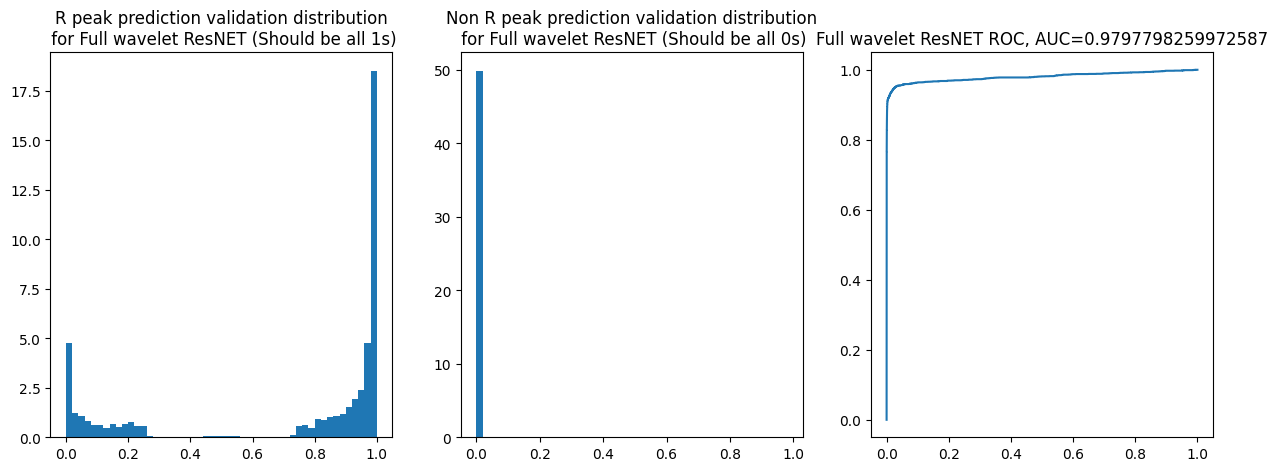
\includegraphics[width=0.75\textwidth]{waveletNetDist.png}
    \caption{Cross-validated predicted values for indicated models.}
\end{figure}

The most glaring difference here is that the standard ResNET model predictions have a lower bound of 0.5 rather than 0. This provides an obvious limitation for predictive accuracy.

Clearly, the Wavelet ResNET model is much more successful at separating the 0 and 1 predictions. Now, let us superimpose the predictions for the 3 block standard ResNET and the 5 layer (32*(block index)  kernel per block) wavelet ResNET model. These models consist of ~2M and ~1.4M trainable parameters respectively, and are thus of a similar order of comlexity.

\begin{figure}[H]
    \centering
    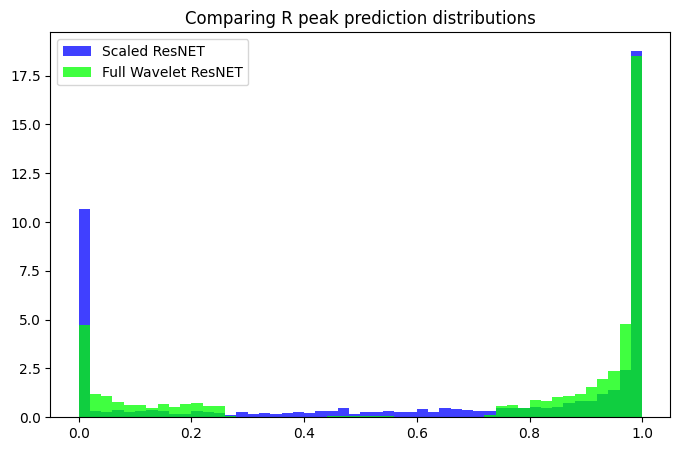
\includegraphics[width=0.45\textwidth]{compRESNETWAVELET.png}
    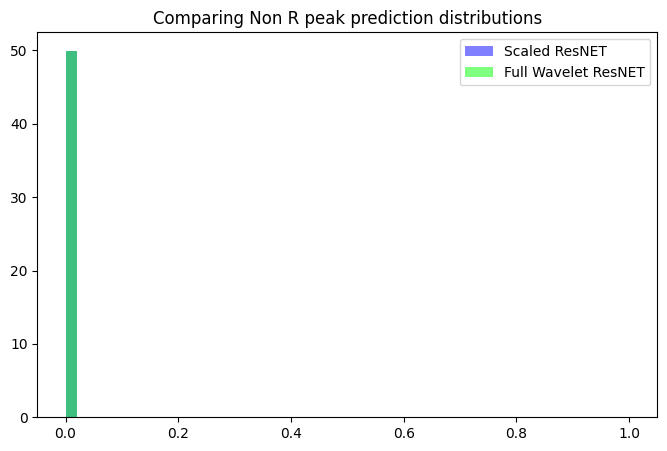
\includegraphics[width=0.45\textwidth]{compRESNETWAVELET_nonr.png}
    \caption{Manually adjusting standard ResNET predictions, and overlaying wavelet ResNET predictions.}
\end{figure}

Even when the standard ResNET outputs are manually normalized to be more favourable, we see that the wavelet ResNET model has more robust performance.

Based on a 95\% bootstrap CI, we can observe that between (26\%,29\%) of cross validated predictions from a wavelet ResNET model are less than 0.5

In contrast, the same interval computed on the standard ResNET gives (33\%,36\%). Therefore, we can conclude that the wavelet is significantly better at correctly identifying R peaks, \textbf{even when the standard wavelet outputs are manually normalised}.

We also see that there is a clearer visual separation of the wavelet ResNET predictions on the true R peaks. The predictions on the rest of the signals coincide almost perfectly for both models. While ideally the models should be predicting all 1 values for the validation R peaks, this is potentially a positive indication that the wavelet model has intrinsically higher capability to form a clearer decision boundary.

It is worth again noting that this wavelet model contained ~1.4M trainable parameters, to teh standard model's ~2M - highly suggestive that the wavelet structure is an inherently more stable and accurate architecture for this specific problem.

\paragraph{\textbf{Comparing Simpler Wavelet Models}}
To be added, shortly


\section{Summary \& Conclusions}

\begin{enumerate}
    \item We have considered an arbitrary neural network layer that attempts to for a decision threshold, above and below which it is conditionally independent of varaitions in the data. We have shown that such a layer cannot both fully respect this property, and be gradient-optimisable. The choice of activation function is what dictates this tradeoff, with a linear relationship between the lower-limit on the gradient of the activation function, and the degree of its unbounded
    \item We have shown how this problem extends to multi-layer neural networks
    \item We have demonstrated that batch normalisation corresponds to the construction of an \textit{adaptive threshold} for this decision boundary, and that it does not eliminate or the above issue
    \item We have proposed a general form of piecewise activation function that allows for the manual tuning of this trade-off
    \item We have explored the similarity between dilated connections in CNN models and the algorithme à trous, and noted how these lead to shift invariant layers
    \item We have described ECG signals in terms of their characteristics time series. We considered the specific clinical problem of automated R peak extraction, and descried this as a general time series problem. In particular, we focus on the conditional invariance of the outputs, which are purely positional in nature, to local amplitude variations in the input data. This makes the aforementioned thoeroetical principles we derived critical for model design,
    \item We demonstrated that taking a principled approach to CNN model design, involving the creation of models that are more cognisant of the above theoretically-derived principles, leads to models that have more accurate and robust predictions, at potentially lower levels of model complexity
\end{enumerate}

\section{Future Research}

\subsection{Further Empirical Experimentation}
The most obvious continuation of this research would be to perform more experiments to further refine our proposed models to attempt to reach state-of-the art, or close to such performance. This could also be attempted for any arbitrary time series problem in any domain, which exhibits the same characteristics as the problem of R peak extraction.

In the context of ECGs, another avenue of potential research is to attempt to generalise our findings to the multivariate case - such as when we need to extract other temporal components in a conditionally amplitude invariant manner, such as T and S waves. This would require consideration of the most robust way to deal with the relationships \textbf{between} these features, which may require a significant extension of the principles and architectures that we have developed here. From this, there is the possibility to consider the problem of QRS complex detection, and the opportunity to benchmark against the many existing approaches to this problem.

\subsection{Generalisation to Filter Banks}
It is worth briefly mention in that in the case, CNN filters are often to be considered as effectively FIR Matched Filters. These produce an amplitude linked to the presence or non-presence of a template signal (the kernel weights). An arbitrary decision boundary learned on these outputs that generate predictions that need to exhibit the same conditional amplitude independence as R peak extraction outputs (i.e., are purely positional outputs), will experience the limitations that we have discussed here. This may potentially have very widespread consequences for CNN models applied to time series problems with very minimal sets of assumptions - which could be a serious issue. This warrants further investigation.

\subsection{Non-positional Time Series Characteristics}
By our restriction to the specific issue of conditional amplitude invariance, we have largely neglected to discuss morphological characteristics of signals/time series, and the capabilities of CNNs for such feature extraction.

There are many potential explorations in this area that could lead to powerful, robust models for different classes of problems in a similar vein to our work here. These may include, but are by no means limited to
\begin{enumerate}
    \item The use of distance measures other than convolution/cross-correlation for Matched Filters
    \begin{itemize}
         \item DTW filters for problems involving local scaling invaraince
         \item Normalised cross correlation for better amplitude invariance
        \end{itemize}
    \item The potential correspondences between Filter Banks (similar to wavelet decompositions) to CNN architectures
    \item The potential correspondences between clustering algorithms, particularly K-Shape\cite{paparrizos2015k} clustering and modified CNN architecutres
    \item Potential benefits of incorporating frequency-domain methods to CNN architectures (other than wavelet transforms), particularly Hilbert-Huang trasnforms
    \item The fundamental limitations of CNN models to extract features that correspond to exact temporal intervals
\end{enumerate}

Finally, once multiple such similar studies are cmopleted, an important area of research would be to investigate the interaction of such models - especially how the stacking or linking of such models affects their convergence and performance.

\section{Acknowledgements}
I would like to thank the staff of the University College Cork Schools of Mathematical Sciences and Computer Science for outstanding tuition and support over the course of my degree.

\vspace{0.5cm}

In particular, I'd like to note my thanks to Professor Gregory Provan, without whose endless patience and support this project would never have come close to starting successfully, much less progressing anywhere.


\bibliographystyle{IEEEtran}
\bibliography{references}

\section{Appendix A: CNN Architectures}

\begin{figure}[H]
    \centering
    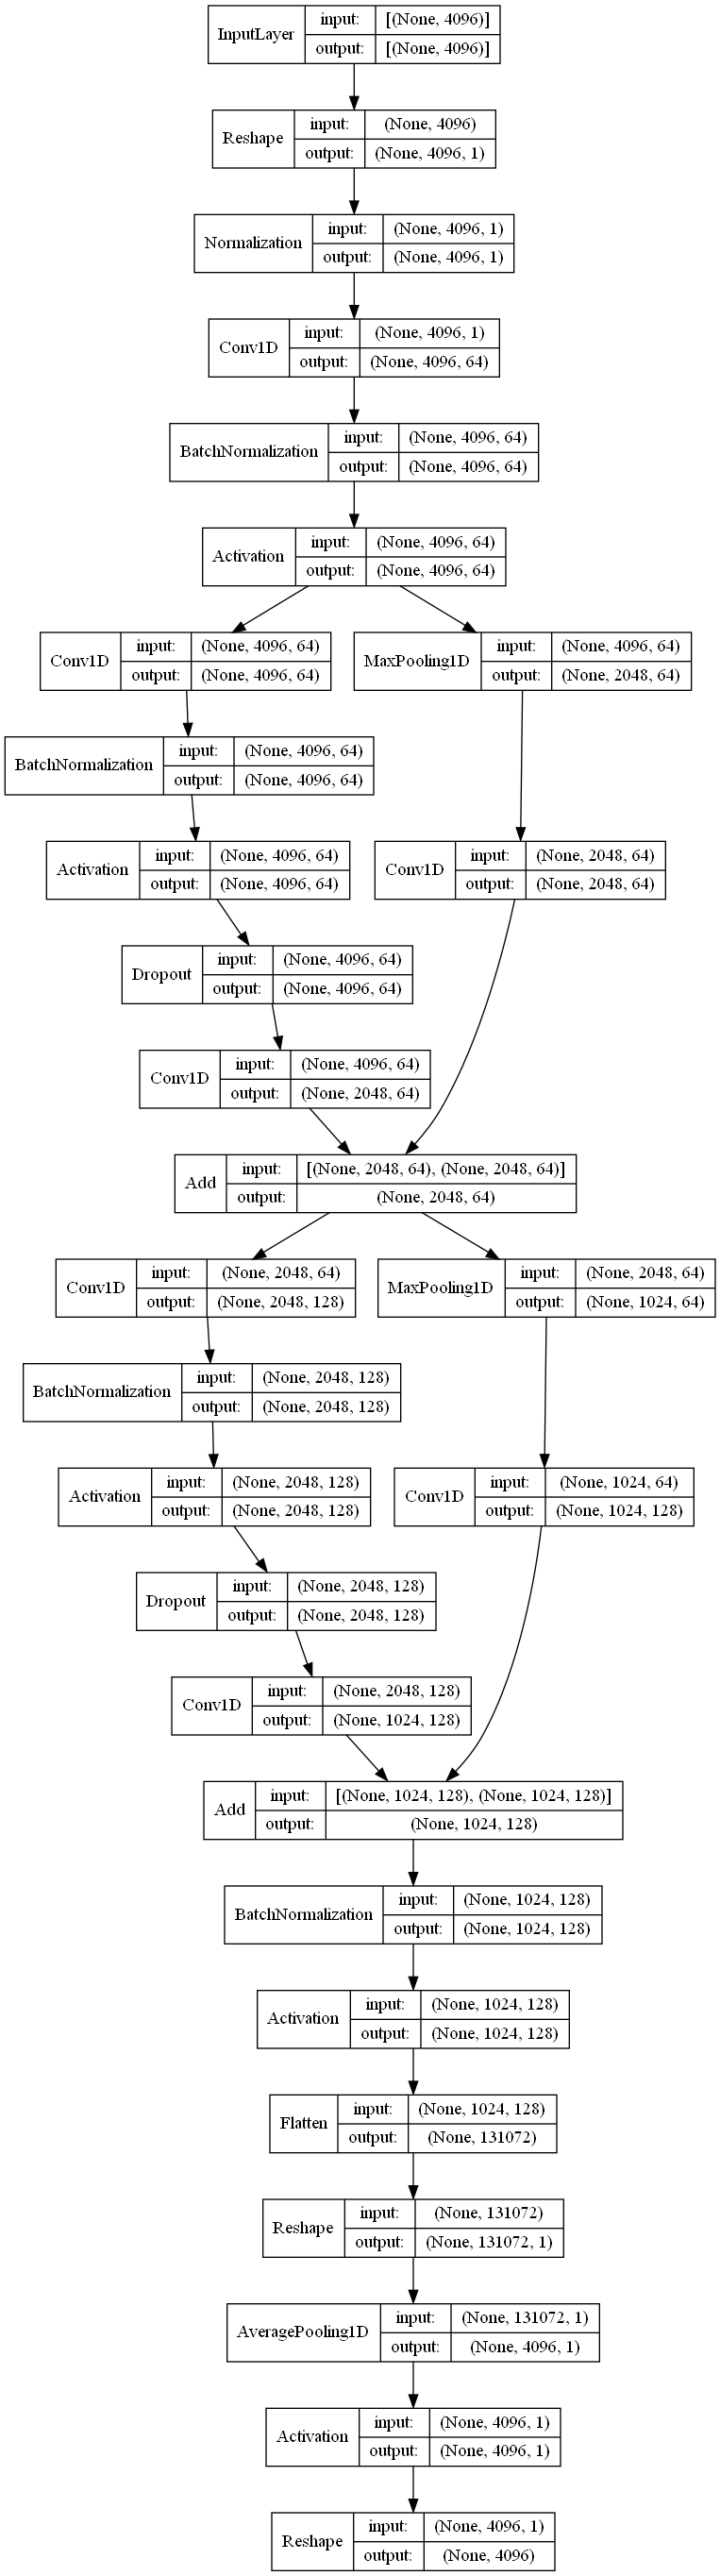
\includegraphics[width=0.35\textwidth]{stanfordmod.png}
    \caption{Conventional Resiudal CNN model, with two residual blocks shown}
\end{figure}

\begin{figure}
    \centering
    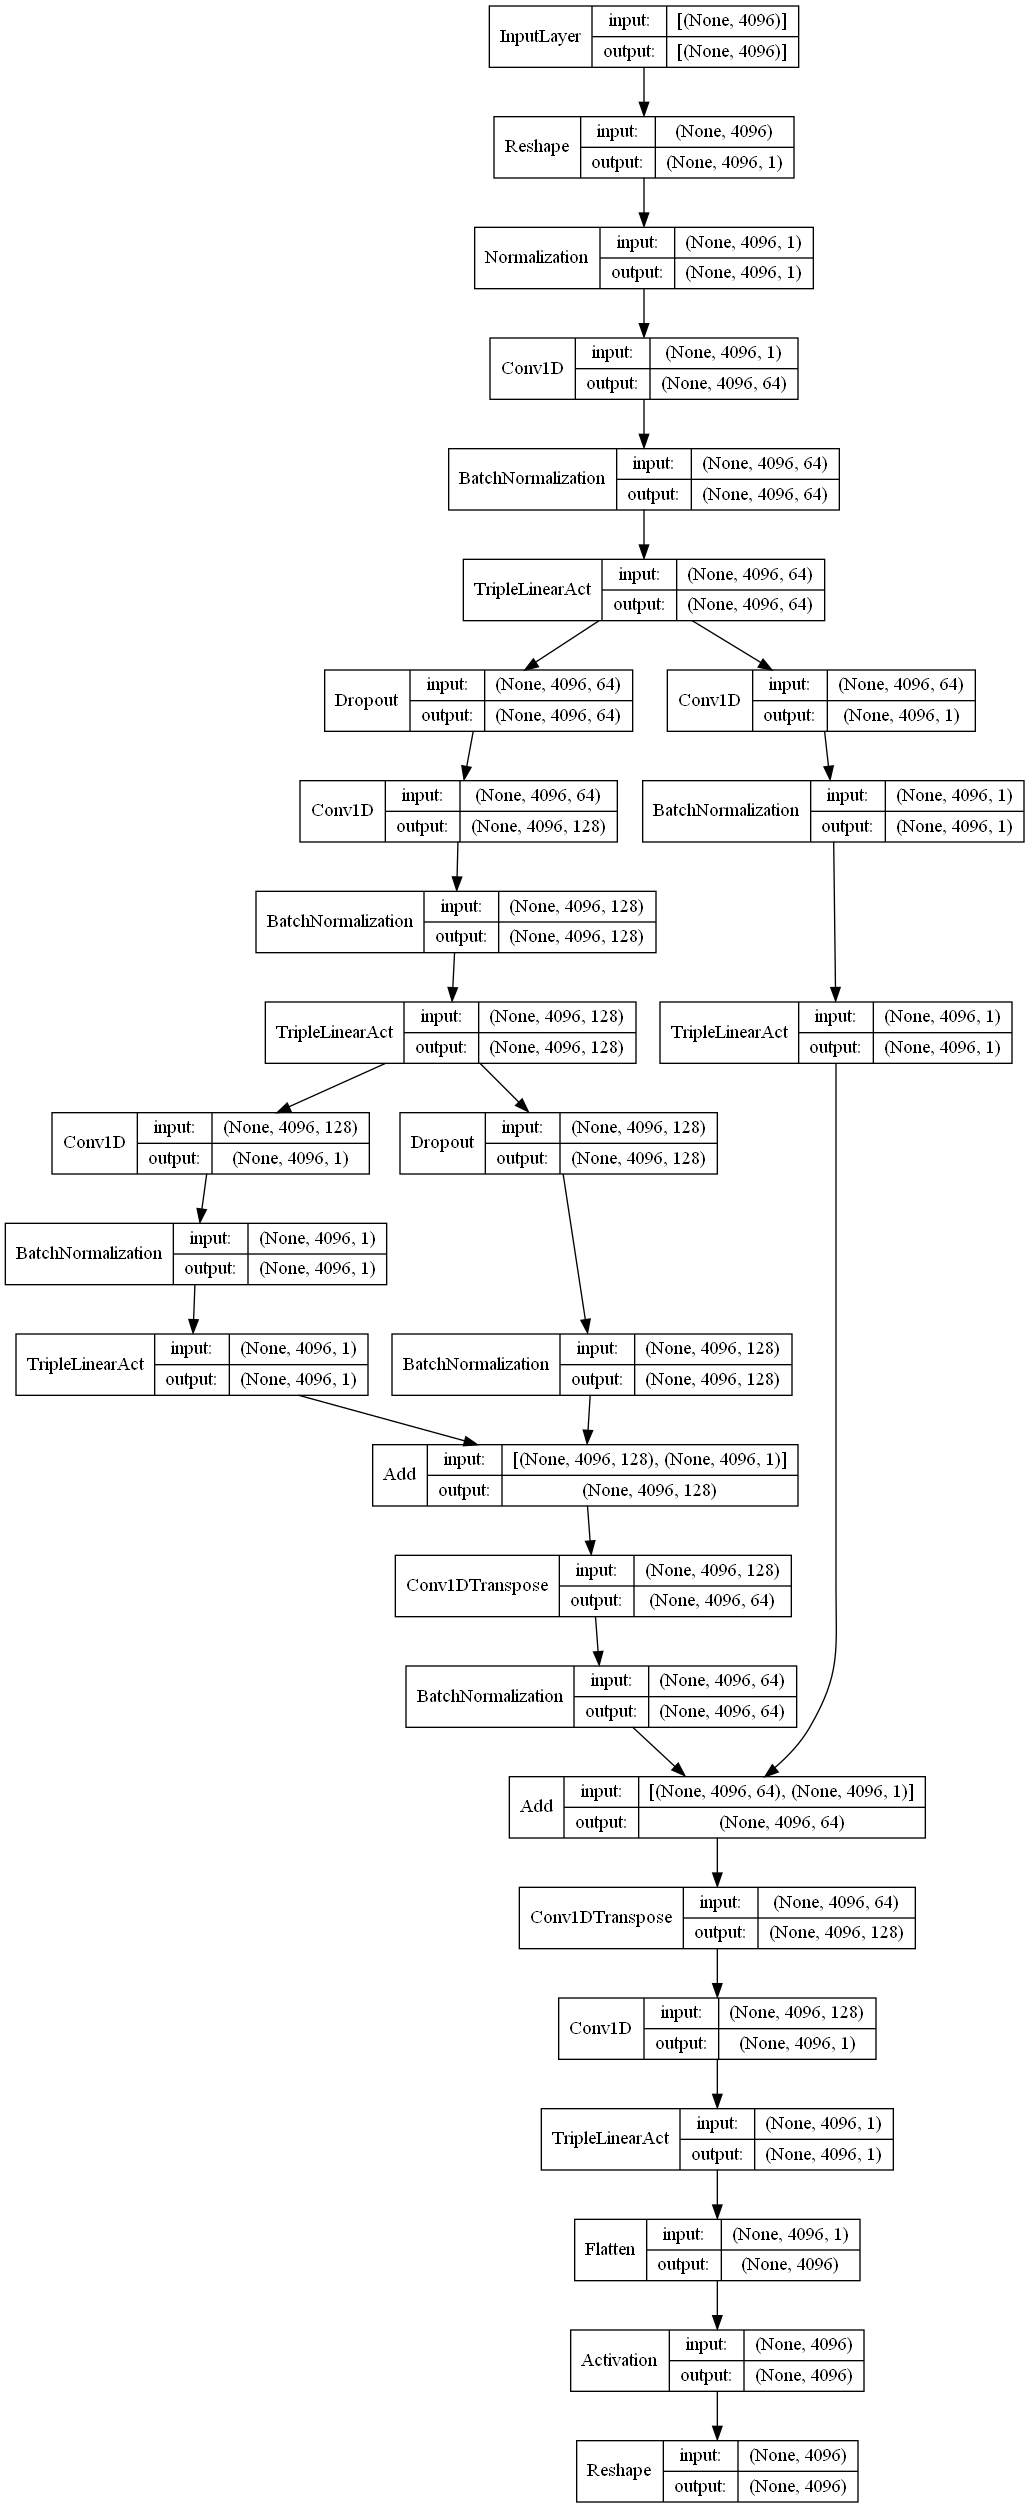
\includegraphics[width=0.5\textwidth]{wavelet_resid.png}
    \caption{Hybrid wavelet-residual CNN model, with two levels of decomposition (and recomposition) shown}
\end{figure}

\clearpage

\section{Declaration of Originality}

In signing this declaration, you are conforming, in writing, that the submitted work is entirely your own original work, except where clearly attributed otherwise, and that it has not been submitted partly or wholly for
any other educational award.

I hereby declare that:

\begin{itemize}
    \item This is all my own work, unless clearly indicated otherwise, with full
and proper accreditation;
    \item With respect to my own work: none of it has been submitted at any educational institution contributing in any way to an educational award;
    \item With respect to another’s work: all text, diagrams, code, or ideas, whether verbatim, paraphrased or otherwise modified or adapted, have been duly attributed to the source in a scholarly manner, whether
from books, papers, lecture notes or any other student’s work, whether published or unpublished, electronically or in print.
\end{itemize}

\vspace{5cm}

\begin{tabular}{@{}p{.5in}p{2in}p{.5in}p{2in}@{}}
Signed: & \hrulefill  & Date &  \hrulefill  \\
& Andrew Nash & &\\
& BSc Data Science \& Analytics & &\\
\end{tabular}


\end{document}

